\section{Spazi metrici e normati}
\subsection{Norme e metriche}

\begin{definition}
	
	$X$ spazio vettoriale su $\mathbb{R}$ o $\mathbb{C}$. Una norma su $X$ è una funzione $\parallel \cdot \parallel : X \rightarrow \mathbb{R}$ tale che 
	\begin{enumerate}
		\item $\parallel x \parallel \geq 0 \quad \forall \ x \in X$ e $\parallel x \parallel = 0 \iff x = 0$
		
		\item $\parallel \lambda x \parallel = |\lambda| \parallel x \parallel \quad \forall$ scalare $\lambda$ e $\forall \ x \in X$
		
		\item $\parallel x+y \parallel \leq \parallel x \parallel + \parallel y \parallel \quad \forall x,y \in X$ (disuguaglianza triangolare)
	\end{enumerate}
	La coppia ($X,\parallel \cdot \parallel$) si dice spazio normato
\end{definition}


\begin{exbar}
\begin{itemize}
	\item $(\mathbb{R}, |\cdot|)$ è spazio normato
	
	\item $(\mathbb{R}^n, |\cdot|)$ è spazio normato (norma euclidea)
	\begin{gather*}
		\overline{x} = (x_1,...,x_n) \in \mathbb{R}^n
		\\ \big| \overline{x} \big| = \sqrt{\sum_{i=1}^{n }x_i^2}= \sqrt{ \langle \overline{x}, \overline{x} \rangle}
	\end{gather*} 
	
	dove, se $\overline{x} = (x_1,...,x_n)$ e $\overline{y} = (y_1,...,y_n)$
	\begin{gather*}
	\langle  \overline{x}, \overline{y} \rangle = \sum_{i=1}^{n} x_i y_i 
	\\
	\text{prodotto scalare tra } \overline{x} \text{ e } \overline{y}
	\end{gather*}

	\item $(\mathbb{R}^n, \parallel \cdot \parallel_{\infty})$ è spazio normato
	\begin{gather*}
		\overline{x} = (x_1,...,x_n) 
		\\
		\parallel \overline{x} \parallel_\infty = \max_{i=1,...,n} |x_i|
	\end{gather*}
	
	(Per casa dimostrare che è una norma)
	
	\item $(\mathbb{R}^n,\parallel\cdot\parallel_1)$ è spazio normato
	\begin{gather*}
		\overline{x} = (x_1,...,x_n)
		\\
		\parallel \overline{x} \parallel_1 \sum_{i=1}^{n} |x_i| = |x_1| + |x_2| + \ldots + |x_n|
	\end{gather*}
	
	
	Se $n=2$ e $(x,y)\in \mathbb{R}^2$
	\begin{gather*}
		\parallel (x,y) \parallel_\infty = \max \{ |x|,|y| \}
		\\
		\parallel (x,y) \parallel_1 = |x| + |y|
	\end{gather*}
	
	\begin{center}
		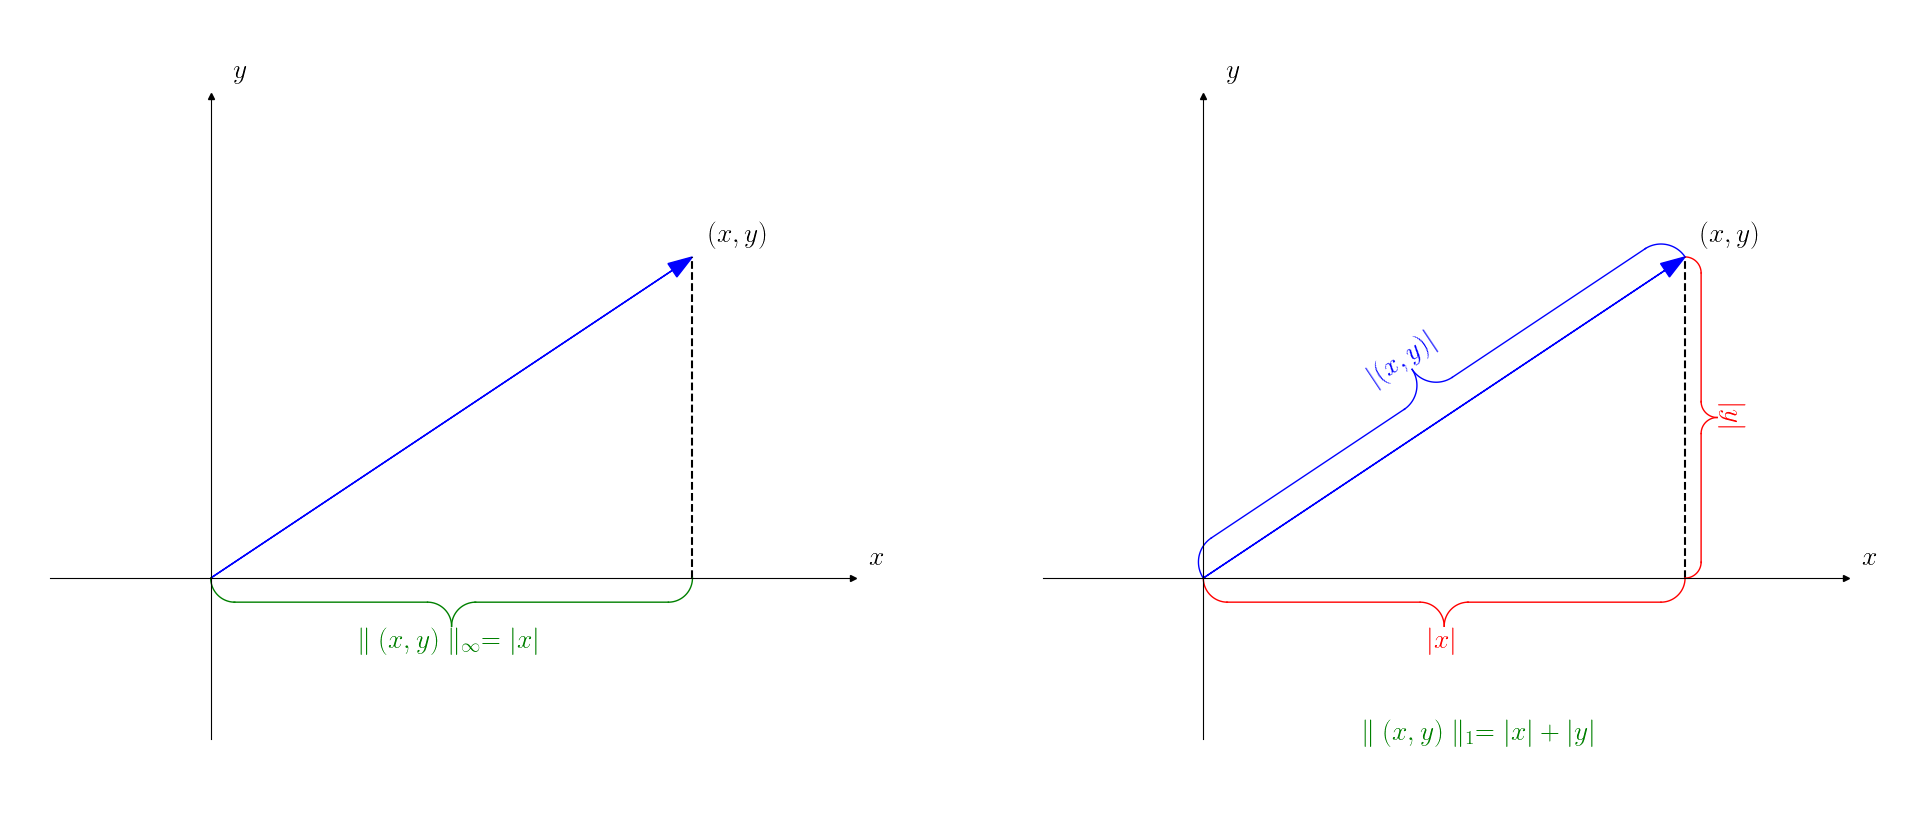
\includegraphics[width=\linewidth]{spazi_metrici_e_normati/pag126}
		\label{fig:pag126}
	\end{center}
	\begin{gather*}
		\parallel \overline{x} \parallel_p = \left( \sum_{i=1}^{n} |x_i|^p \right)^{\frac{1}{p}} \quad p \geq 1
		\\
		\parallel \overline{x} \parallel_\infty = \lim_{p \rightarrow +\infty} \parallel \overline{x} \parallel_p
	\end{gather*}
	$(\mathbb{R}^n, \parallel \cdot \parallel_p)$ è spazio normato

	\item $C^0 \left( [0,1] \right)$
	\begin{align*}
		&\parallel f \parallel_\infty = \sup_{x \in [0,1]} |f(x)| (=\max_{x \in [0,1]} |f(x)|)
		\\
		&\parallel f \parallel_1 = \int_{0}^{1} |f(x)| \ \mathrm{d}x
		\\
		&\parallel f \parallel_p = \left( \int_{0}^{1} |f(x)|^p \ \mathrm{d}x \right)^{\frac{1}{p}} \qquad p \geq 1
	\end{align*}

sono tute norme su $C^0 ([0,1])$
\end{itemize}
\end{exbar}


\begin{exbar}
\begin{example}
	Facciamo vedere che $\parallel \cdot \parallel_\infty$ su $C^0 ([0,1])$ è una norma
	\begin{enumerate}
		\item $\parallel f \parallel_\infty \geq 0 \qquad$ (banale)
		
		$\parallel f \parallel_\infty =  0 \iff f(x) = 0 \qquad \forall \ x \in [0, 1]$
		
		$\parallel f \parallel_\infty =  0 \iff \sup_{x \in [0,1]} |f(x)| = 0$
		
		$\iff 0 \leq |f(x)| \leq 0 \quad \forall \ x \in [0,1] \iff f(x) = 0 \qquad \forall \ x \in [0,1]$
		
		\item $\parallel \lambda f \parallel_\infty = |\lambda| \parallel f \parallel_\infty \qquad \forall \lambda \in \mathbb{R}$ e $\forall f \in C^0 ([0,1])$
		
		$\parallel \lambda f \parallel_\infty = \sup_{x \in[0,1]} |\lambda f(x)| = \sup_{x\in[0,1]} |\lambda| \ |f(x)| = |\lambda| \sup_{x\in[0,1]} |f(x)| = |\lambda| \parallel f \parallel_\infty$
		
		\item $\parallel f+g \parallel_\infty \leq \parallel f \parallel_\infty + \parallel g \parallel_\infty \qquad \forall f,g \in C^0 ([0,1])$
		
		$\parallel f+g \parallel_\infty = \sup_{x\in[0,1]} |f(x) + g(x)|$
		
		$|f(x) + g(x)| \distr |f(x)| + |g(x)| \leq \sup_{y\in[0,1]} |f(y)| + \sup_{y\in[0,1]} |g(y)| =  \parallel f \parallel_\infty + \parallel g \parallel_\infty \qquad \forall \ x \in [0,1]$
		
		$\parallel f+g \parallel_\infty = \sup_{x\in[0,1]} |f(x) + g(x)| \leq \parallel f \parallel_\infty + \parallel g \parallel_\infty$\\
	\end{enumerate}
\end{example}
\end{exbar}
	

\begin{exbar}
\begin{example}
		Facciamo vedere che $\parallel f\parallel_1 = \int_{0}^{1} |f(x)| \ \mathrm{d}x$
		
		è una norma
	\begin{enumerate}
		\item $\parallel f \parallel_1 \geq 0 \qquad \forall f \in C^0 ([0,1]) \text{ banale}$
		
		Dimostriamo che $\parallel f \parallel_1 = 0 \iff f(x) = 0 \qquad \forall \ x \in [0,1]$
		
		$\Leftarrow) f(x) = 0 \qquad \forall \ x \in[0,1]$
		
		$\parallel f \parallel_1 = \int_{0}^{1} 0 \ \mathrm{d}x = 0$
		
		$\Rightarrow)$ Sia $\parallel f \parallel_1 = 0$ e dimostriamo che $f(x) = 0 \qquad \forall \ x \in [0,1]$
		
		$\int_{0}^{1} |f(x)| \ \mathrm{d}x = 0$
		
		Se $\exists \ x_0 \in [0,1]$ tale che $|f(x_0)| \neq 0$ allora $\exists$ un intorno $U$ di $x_0 $ tale che $|f(x)| \geq \frac{|f(x_0)|}{2}$ $\qquad \forall x \in U \cap [0,1]$ 
		
		\begin{itemize}
			\item $U = \ ]x_0 - \delta, x_0 + \delta[ \ \subseteq [0,1]$
	
			\item $x_0=0$
			
			$U= \ ]0 - \delta, 0 + \delta[$
			
			$U \cap [0,1] = [0, \delta[$
			
			\item $x_1 = 1$
			 $U= \ ]1 - \delta, 1 + \delta[$
			 
			$U \cap [0, 1] = \ ]1 - \delta, 1]$
		\end{itemize}
		
		cioè in ogni caso $U \cap [0,1]$ è un intervallo di ampiezza almeno $\frac{\delta}{2}>0$
		
		\begin{equation*}
			\parallel f\parallel_1 = \int_{0}^{1} |f(x)| \ \mathrm{d}x \geq \int_{U \cap [0,1]} |f(x)| \ \mathrm{d}x \geq \int_{U \cap [0,1]} \frac{|f(x_0)|}{2} \ \mathrm{d}x \geq \frac{\delta}{4} |f(x_0)| > 0
		\end{equation*}
		
		il che è assurdo, perché $\parallel f\parallel_1 = 0$
		
		\item $\parallel \lambda f \parallel_1 = \int_{0}^{1} |\lambda f(x)| \ \mathrm{d}x = |\lambda| \int_{0}^{1} |f(x)| \ \mathrm{d}x = |\lambda| \parallel f \parallel_1 \qquad \lambda \in \mathbb{R}$
		
		\item $f,g \in C^0 ([0,1])$
		
		$\parallel f+g \parallel_1 = \int_{0}^{1} |f(x) + g(x)| \ \mathrm{d}x \leq \int_{0}^{1} (|f(x)| + |g(x)|) \ \mathrm{d}x = \parallel f \parallel_1 + \parallel g \parallel_1$
		
		$\Rightarrow$ vale la disuguaglianza triangolare
	\end{enumerate}
\end{example}
\end{exbar}


\begin{attbar}
	Dato uno spazio normato $(X, \parallel \cdot \parallel)$ posso definire la distanza tra due vettori $x,y \in X$ come $d(x,y)= \parallel x-y \parallel$, lunghezza del vettore $x-y$
	\begin{center}
		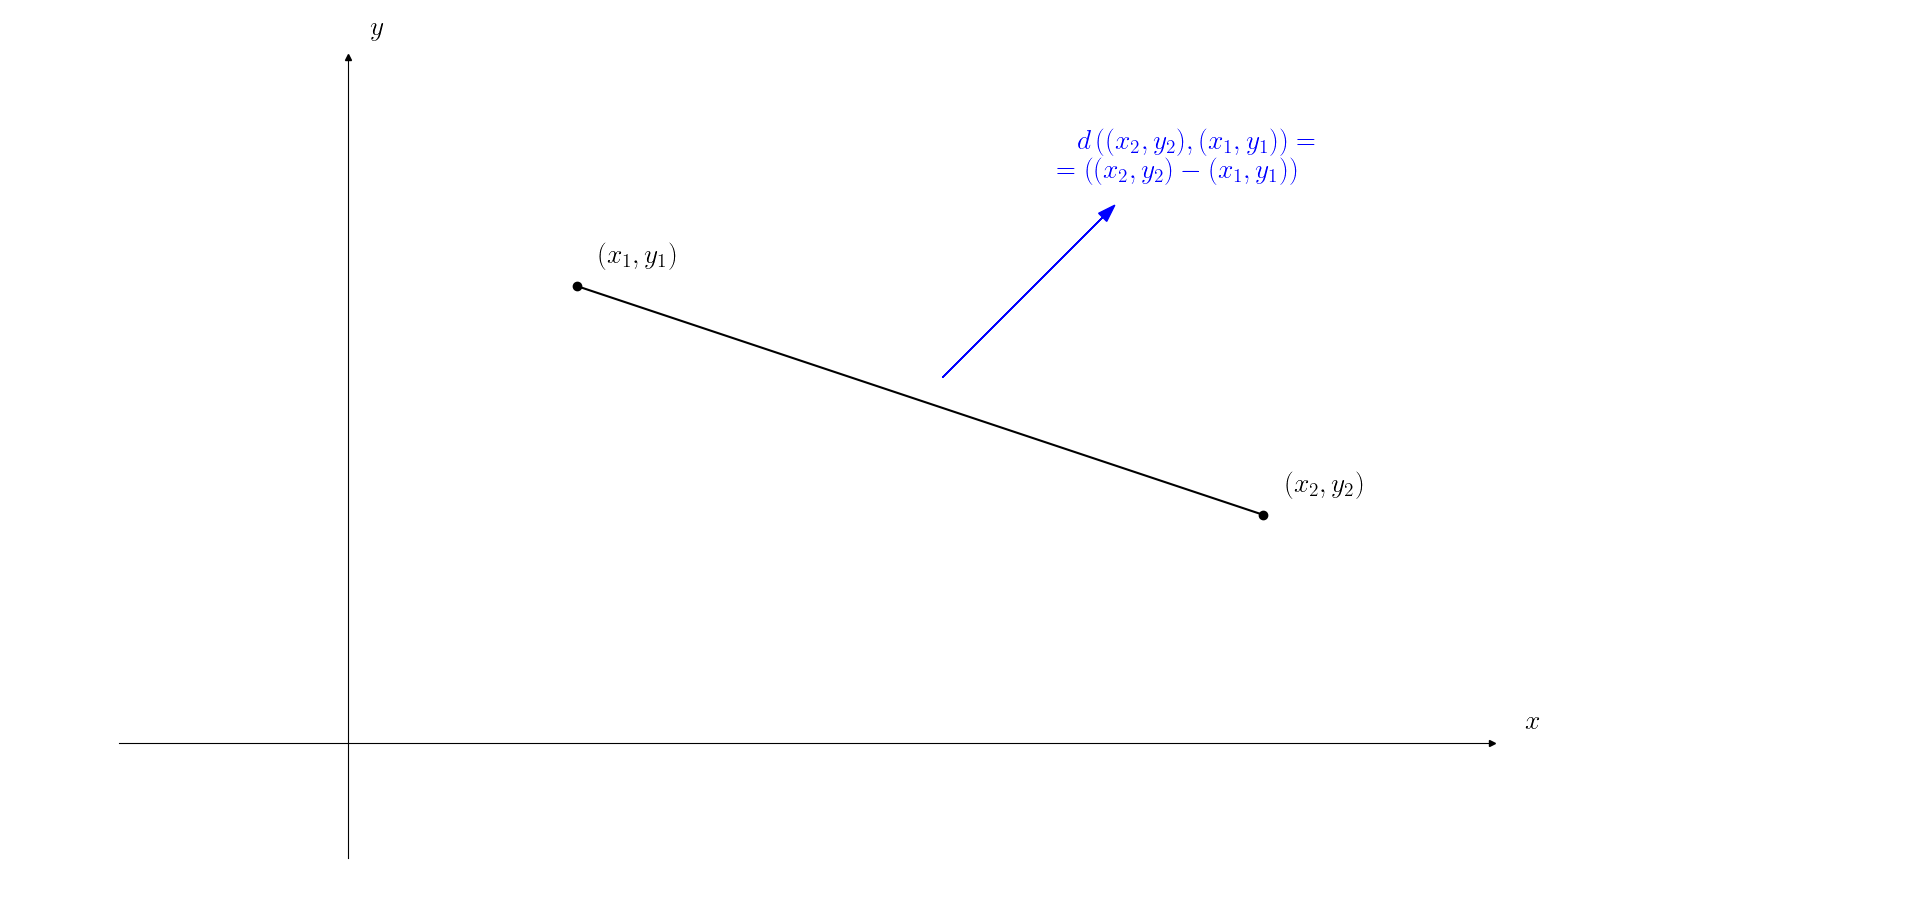
\includegraphics[width=0.75\linewidth]{spazi_metrici_e_normati/pag131}
		\label{fig:pag131}
	\end{center}
\end{attbar}


\begin{definition}
	$X$ insieme non vuoto. Una distanza o metrica su $X$ è una funzione $d:X \times X \rightarrow \mathbb{R}$ tale che
	\begin{enumerate}
		\item $d(x,y) \geq 0 \qquad \forall \ x,y \in X $ e $d(x,y) = 0 \iff x = y$
		\item $d(x,y) = d(y,x)$ (proprietà simmetrica)
		\item Disuguaglianza triangolare $d(x,y) \leq d(x,z) + d(z,y) \qquad \forall \ x,y,z \in X$
	\end{enumerate}
	
	La coppia $(X,d)$ si dice \textbf{spazio metrico}.
\end{definition}



$(X, \parallel \cdot \parallel)$ normato

$d(x,y)=\parallel x-y \parallel$ è metrica, allora
\begin{enumerate}
	\item $d(x,y)\geq 0$ banalmente 
	$d(x,y) = \parallel x-y \parallel = 0 \iff x-y = 0 \iff x = y$
	\item $d(x,y) = \parallel x-y \parallel = \parallel y-x \parallel = d(y,x)$
	\item $d(x,y) = \parallel x-y \parallel = \parallel (x-z) + (z-y) \parallel \leq \parallel x-z \parallel + \parallel z-y \parallel = d(x,z) + d(y,z)$
\end{enumerate}

Dato uno spazio vettoriale $X$ e $d$ metrica su $X$, esiste una norma $\parallel \cdot \parallel$ su $X$ tale che $d(x,y) = \parallel x-y \parallel$?

No, esistono metriche dentro lo spazio vettoriale che non derivano da una norma.


\begin{exbar}
\begin{example}
	$\mathbb{R}, \quad 0 < p < 1 , \quad d(x,y) = |x-y|^p$. 
	
	Allora $d$ è una metrica, che non deriva da una norma.
	
	Se esistesse una norma $\parallel \cdot \parallel$ su $\mathbb{R}$ tale che $d(x,y) = \parallel x-y \parallel$, allora, fissato $\lambda \in \mathbb{R}$,
	\begin{gather*}
		d(\lambda x, \lambda y) = \parallel \underbrace{\lambda x - \lambda y}_{\lambda (x - y)} \parallel \uppercomment{=} {\text{seconda}} {\text{proprietà di }\parallel \cdot \parallel} |\lambda| \parallel x-y \parallel = |\lambda | \ d(x,y)
		\\
		d(\lambda x, \lambda y) = |\lambda x - \lambda y|^p = |\lambda|^p |x-y|^p = |\lambda|^p d(x,y) \neq |\lambda| \ d(x,y) \text{ se } |\lambda \neq 1,0|
	\end{gather*}
	
	Facciamo vedere che $d(x,y) = |x-y|^p$ è una distanza, $0 < p < 1$
	\begin{enumerate}
		\item $d(x,y) \geq 0$ banale
		
		$d(x,y) = 0 \iff |x-y|^p = 0 \iff |x-y| = 0 \iff x = y$
		
		\item $d(x,y) = d(y,x)$ banale
		
		\item Disuguaglianza triangolare
		
		Dobbiamo dimostrare che $\forall \ x,y,z \in \mathbb{R}$ vale
		\begin{gather*}
			d(x,y) \leq d(x,z) + d(z,y)
			\\
			|x-y|^p \leq |x-z|^p + |z-y|^p
			\\
			|x-y|^p \distr (|x-z| + |y-z|)^p
		\end{gather*} 
	
		Se dimostro che $( \underbrace{|x-z|}_{= a} + \underbrace{|y-z|}_{=b})^p \leq |x-z|^p + |z-y|^p$, sono a posto $\forall \ x,y,z \in \mathbb{R}$ con $0<p<1$.
		
		Devo dunque dimostrare che $(a+b)^p \leq a^p + b^p \qquad \forall \ a,b \in \mathbb{R}^{\geq 0}$.
		
		Se $a=0$ o $b=0$, banale
		
		Siano $a,b \neq 0$
		\begin{gather*}
		(a + b)^p \leq a^p + b^p \qquad /.\frac{1}{b^p}
		\\
		\iff \frac{(a+b)^p}{b^p} \leq \frac{a^p}{b^p} + 1 \iff \left( \frac{a+b}{b} \right)^p \leq \left( \frac{a}{b} \right)^p + 1 \iff \left( \frac{a}{b} + 1 \right)^p \leq \left( \frac{a}{b} \right)^p + 1 \qquad \forall \ a,b > 0
		\end{gather*}
		
		Posto $\lambda = \frac{a}{b}>0$
		\begin{gather*}
		\left( \frac{a}{b} + 1 \right)^p \leq \left( \frac{a}{b} \right)^p + 1 \qquad \forall \ a,b>0 \iff (\lambda + 1)^p \leq \lambda^p + 1 \qquad \forall \ \lambda > 0
		\\
		(\lambda + 1)^p - \lambda^p \leq 1
		\\
		f(\lambda) = (\lambda + 1)^p -\lambda^p \qquad f:\mathbb{R}^{\geq 0} \rightarrow \mathbb{R}
		\\
		f(\lambda) \leq 1 = f(0)
		\\
		f'(\lambda) 
		\lowercomment{=} {\myarrow[270]} {\lambda \neq 0} p \ (\lambda + 1)^{p - 1} - p \ \lambda^{p - 1} 
		= p \ [(\lambda + 1)^{p - 1} - \lambda^{p - 1}] 
		= p \ \lambda^{p - 1} \left[ \left( \frac{\lambda + 1}{\lambda} \right)^{p-1} - 1 \right] 
		\\
		=  p \ \lambda^{p - 1} \left[ \underbrace{ \left(  1 + \frac{1}{\lambda} \right) ^{\overbrace{p - 1}^{<0}} }_{<1} - 1 \right] < 0 \qquad \forall \ \lambda > 0
 		\end{gather*}
		
		$f$ è decrescente e quindi $\forall \ \lambda > 0 \Rightarrow f(\lambda) \leq f(0)$, come si voleva.
	\end{enumerate}
\end{example}
\end{exbar}


\subsection{Topologia}

$(x,d)$ spazio metrico.

\begin{definition}
	
\end{definition}
	Sia $x \in X, r >0$, allora $B_r(x) = \{ y \in X | d(x,y) < r \}$ si dice \textbf{palla (aperta)} di centro $x$ e raggio $r$.

	
\begin{exbar}
	\begin{gather*}
		(\mathbb{R}^2, | \cdot |), \qquad \mathbb{R}^2 \text{ con norma euclidea}
		\\
		B_r (0,0), \qquad r > 0
		\\
		B_r (0,0) 
		= \{ (x,y) \in \mathbb{R}^2 \big| d((x,y), (0,0)) < r \} 
		= \{ (x,y) \in \mathbb{R}^2 \big| |(x,y)-(0,0)| < r \} =
		\\ 
		= \{ (x,y) \in \mathbb{R}^2 \big| \sqrt{x^2+y^2} < r\}
	\end{gather*}
	\begin{center}
		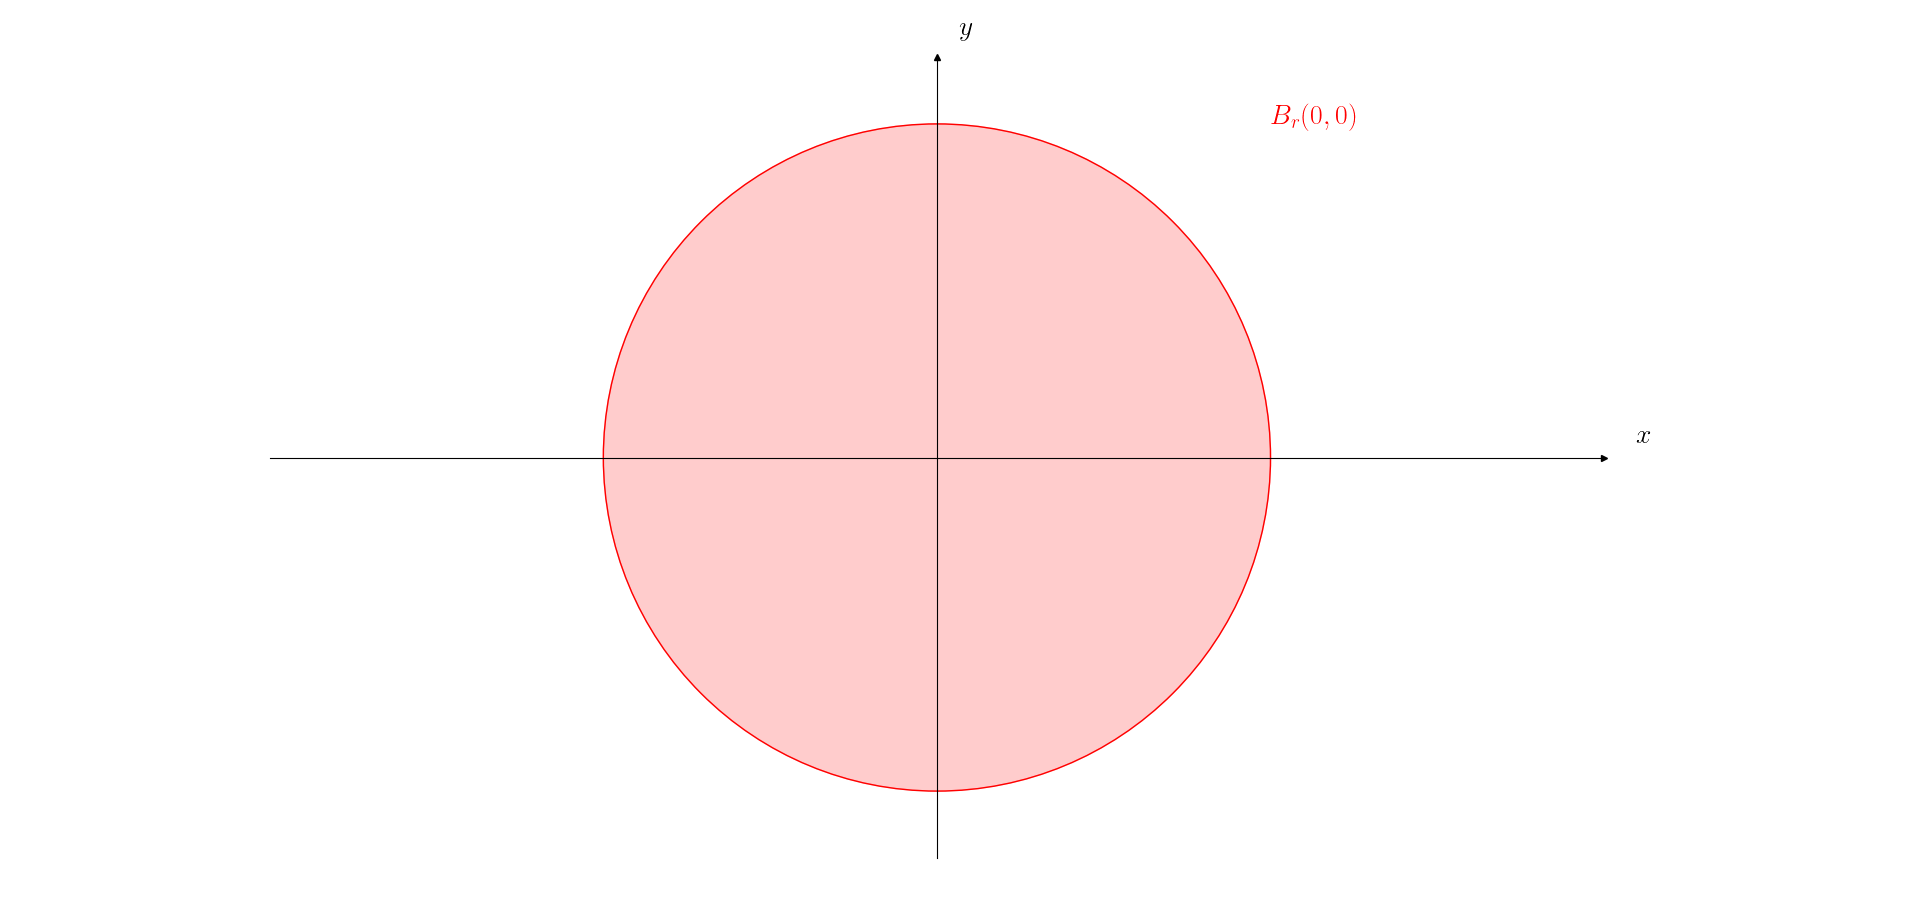
\includegraphics[width=0.75\linewidth]{spazi_metrici_e_normati/pag137circle}
		\label{fig:pag137circle}
	\end{center}
	
	\begin{gather*}
	 	(\mathbb{R}^2, \parallel \cdot \parallel_\infty)
	 	\\
		\parallel (x,y) \parallel_\infty = \max \{|x|,|y|\} 
		\\
		B_r^\infty (0,0) 
		= \{ (x,y) \in \mathbb{R}^2 \big| \parallel(x,y) - (0,0) \parallel_\infty < r \} 
		= \{ (x,y) \in \mathbb{R}^2 \big| \max \{|x|,|y| \} < r \} =
		\\
		= \{ (x,y) \in \mathbb{R}^2 \big| |x|,|y| < r\}
	\end{gather*}
	\begin{center}
		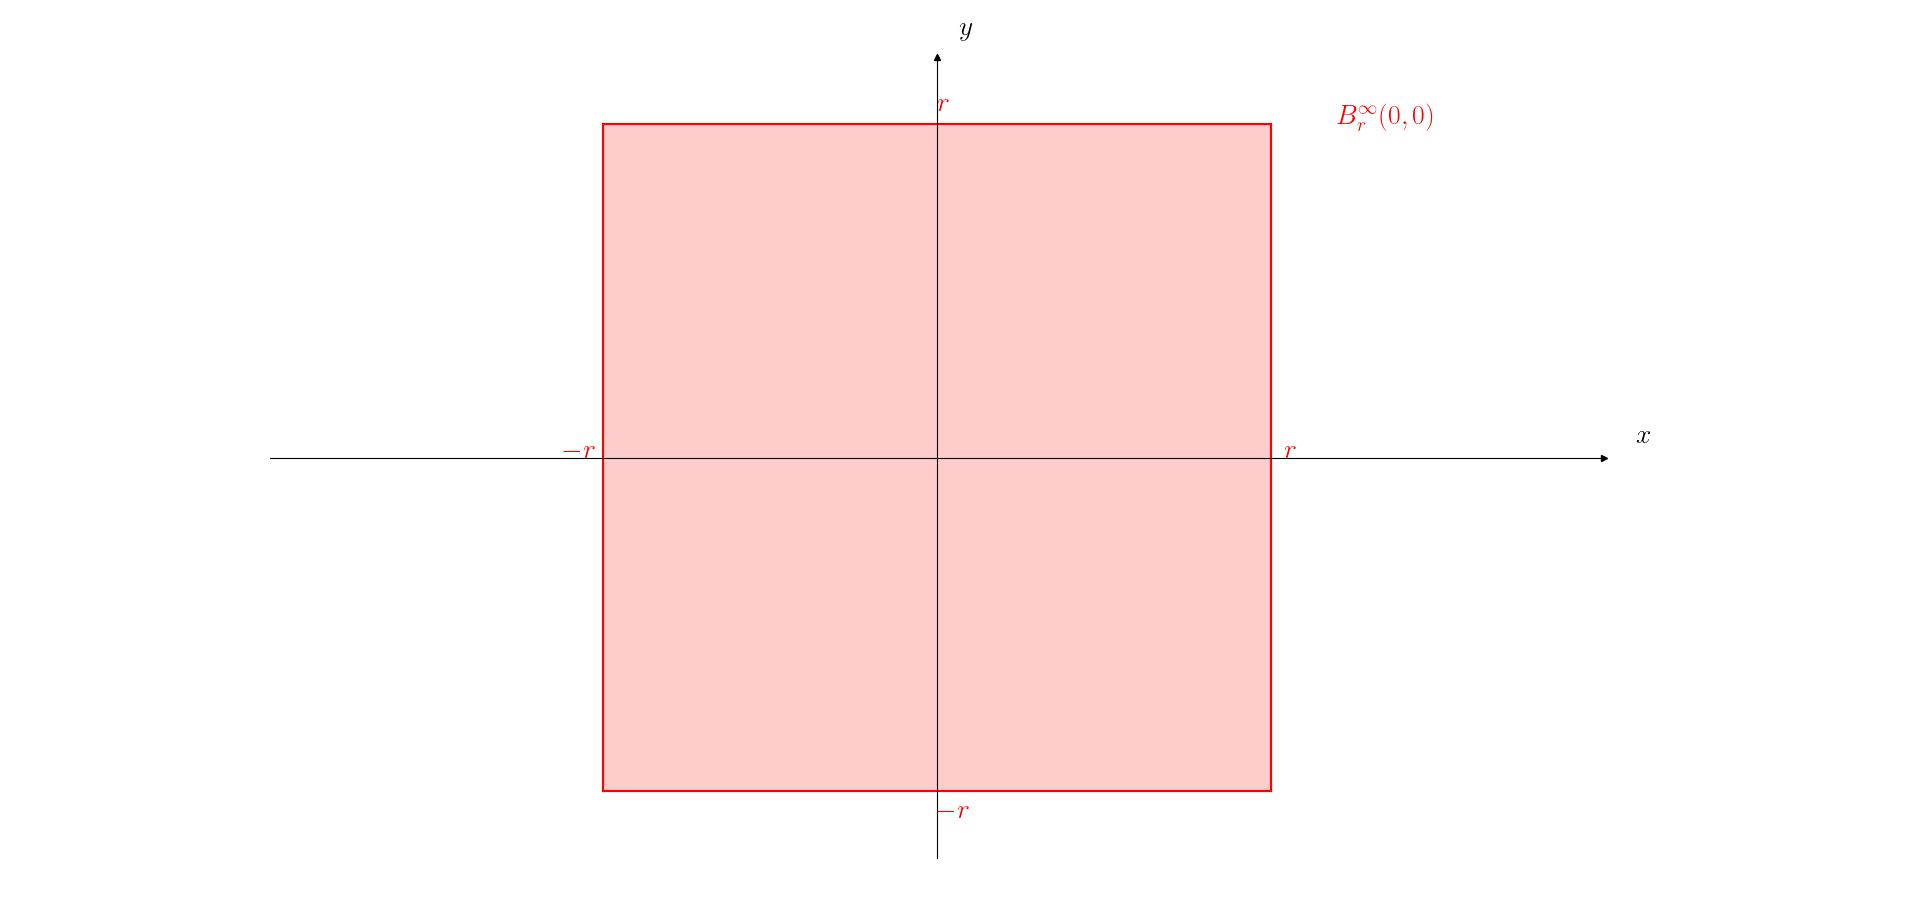
\includegraphics[width=0.75\linewidth]{spazi_metrici_e_normati/pag137square}
		\label{fig:pag137square}
	\end{center}
	
	\begin{gather*}
		(\mathbb{R}^2, \parallel \cdot \parallel_1)
		\qquad
		\parallel (x,y) \parallel_1 = |x| + |y| 
		\\
		B_r^1 (0,0) = \{(x,y) \in \mathbb{R}^2 \big| \parallel (x,y) - (0,0) \parallel_1 < r \} 
		= \{(x,y) \in \mathbb{R}^2 \big| |x| + |y| < r \}
	\end{gather*}
	\begin{center}
		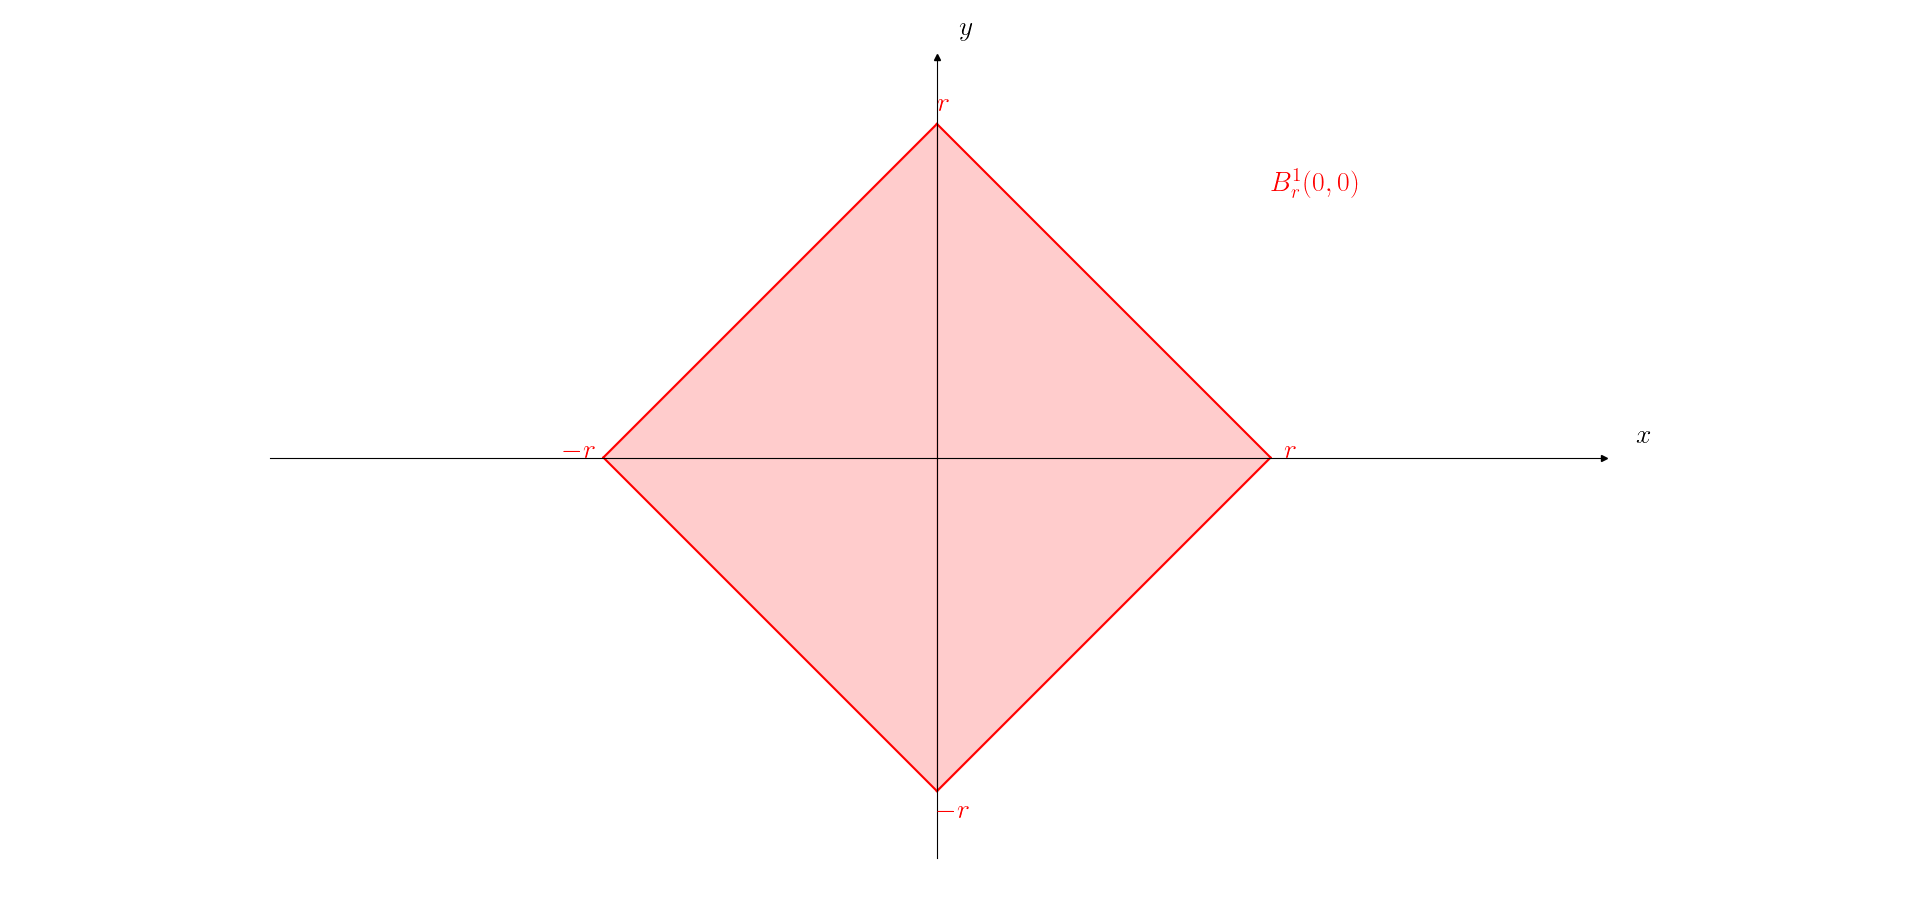
\includegraphics[width=0.75\linewidth]{spazi_metrici_e_normati/pag138rhombus}
		\label{fig:pag138rhombus}
	\end{center}

	\begin{gather*}
		(C^\circ([0,1]), \parallel \cdot \parallel_\infty) \qquad
		d(f,g) = \parallel f-g \parallel_\infty
		\\
		f \in C^0 (), \qquad r>0
		\\
		B_r^\infty(f) = \{ g \in C^0 ([0,1]) \big| \parallel f-g \parallel_\infty < r \} = \{ g \in C^0 ([0,1]) \big| \undercomment{\sup_{x \in [0,1]} |f(x) - g(x)|} {f(x) - r < g(x) < f(x) + r} {} < r \} 
	\end{gather*}		
	\begin{center}
		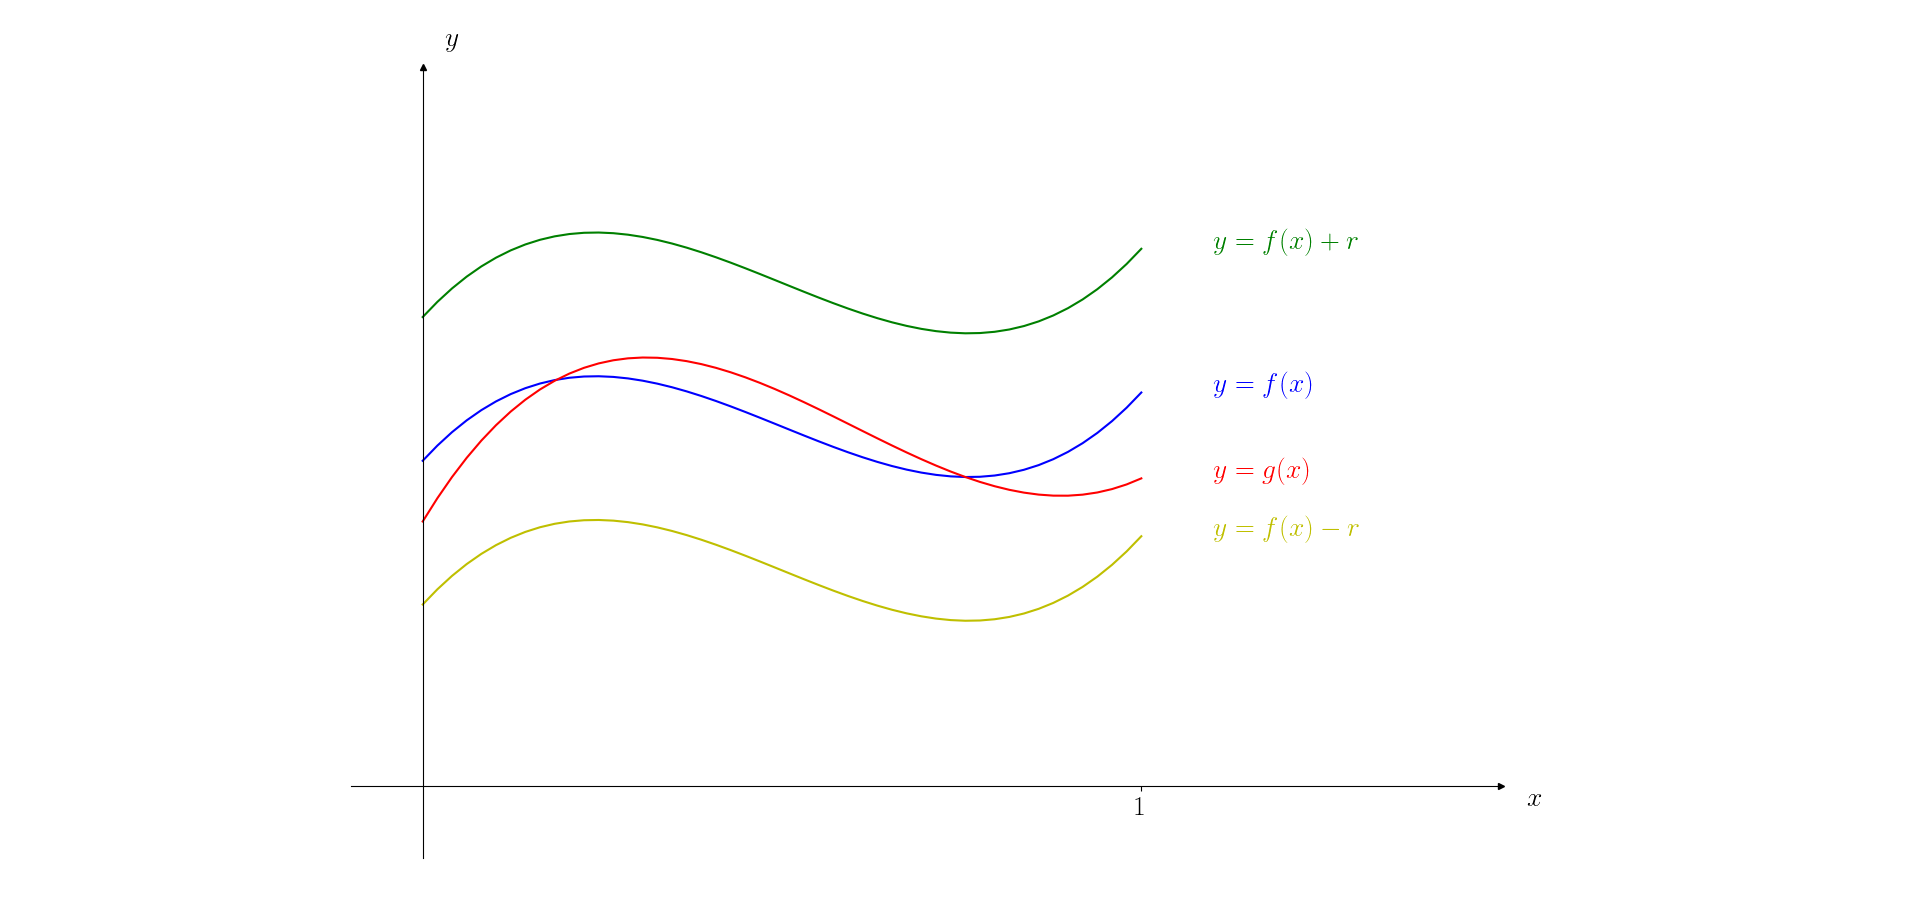
\includegraphics[width=0.75\linewidth]{spazi_metrici_e_normati/pag138curve}
		\label{fig:pag138curve}
	\end{center}
	
	$$f(x)=0 \qquad \forall \ x \in [0,1]$$
	\begin{center}
		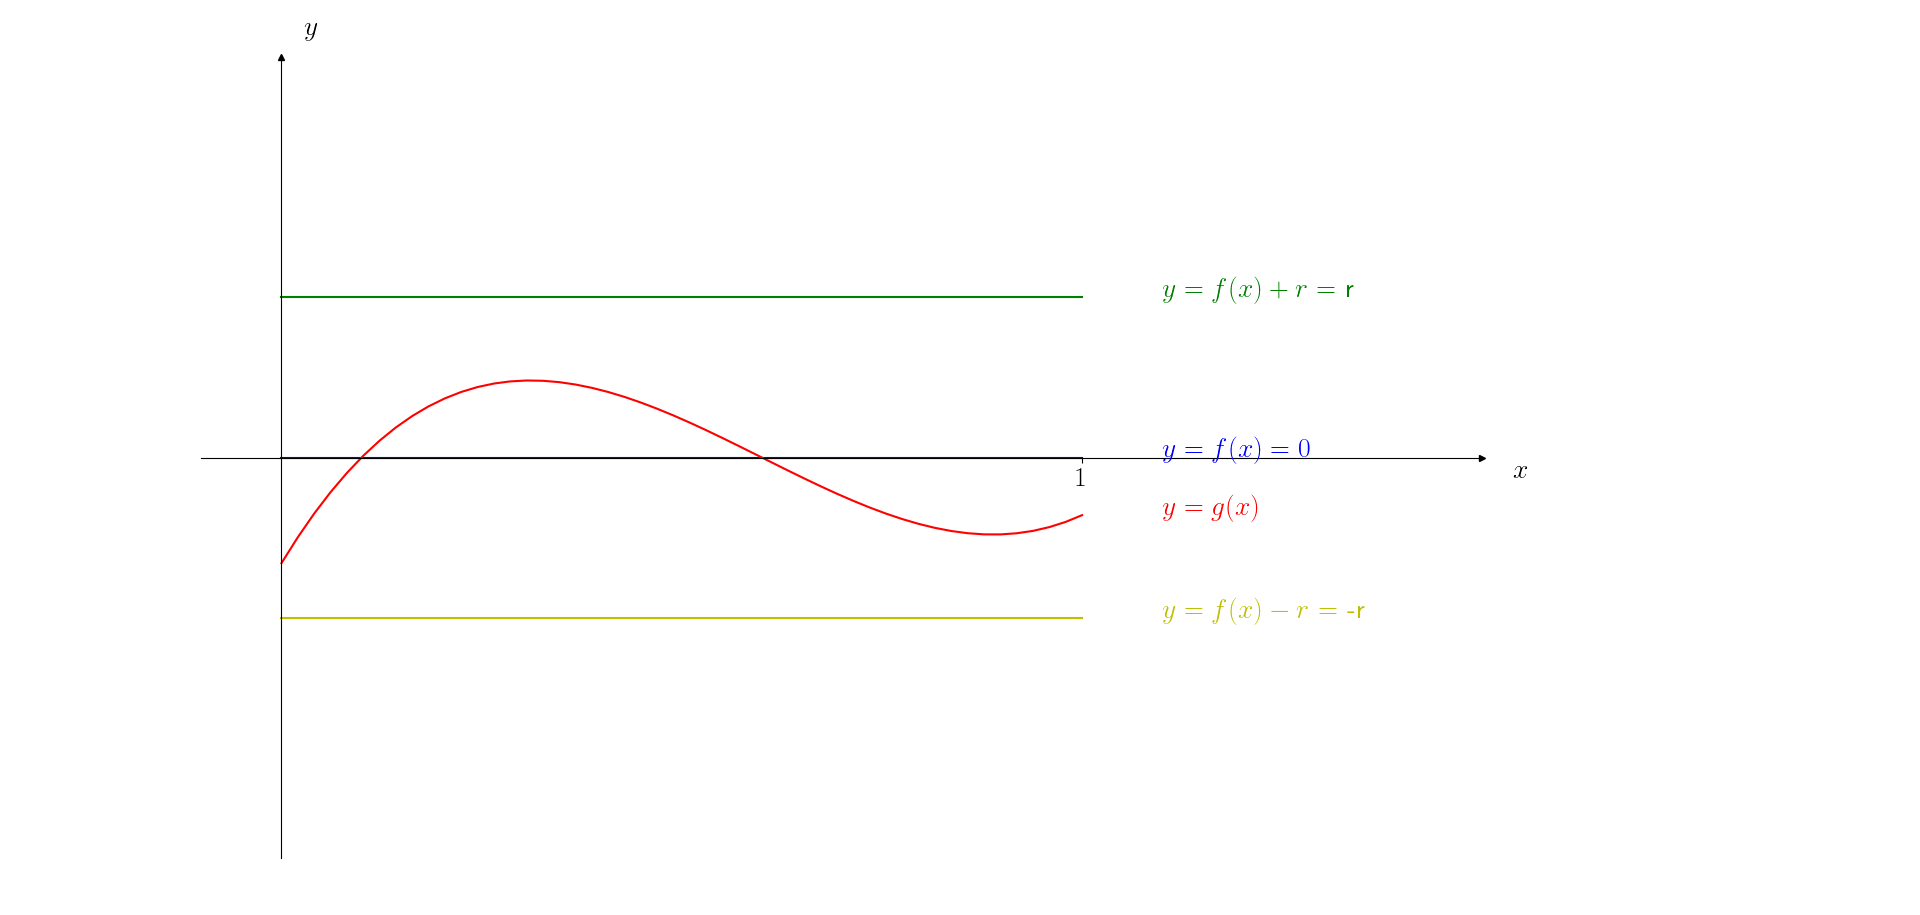
\includegraphics[width=0.65\linewidth]{spazi_metrici_e_normati/pag139curve}
		\label{fig:pag139curve}
	\end{center}
	
	\begin{gather*}
		C^0 ([0,1]), \parallel \cdot \parallel_1
		\\
		\parallel f \parallel_1 = \int_{0}^{1} |f(x)| \ \mathrm{d}x 
		\\
		B_r^1 = \{ g \in C^0 ([0,1]) \big| \parallel f-g \parallel_1 < r \} = \{g \in C^0 ([0,1]) \bigg| \int_{0}^{1} |f(x) - g(x)| \ \mathrm{d}x < r \}
		\\
		f(x) = 0 \qquad \forall \ x \in [0,1]
		\\
		B_r^1(0) = \{ g \in C^0 ([0,1]) \bigg| \int_{0}^{1} |g(x)| \ \mathrm{d}x < r \}
	\end{gather*}
	\begin{center}
		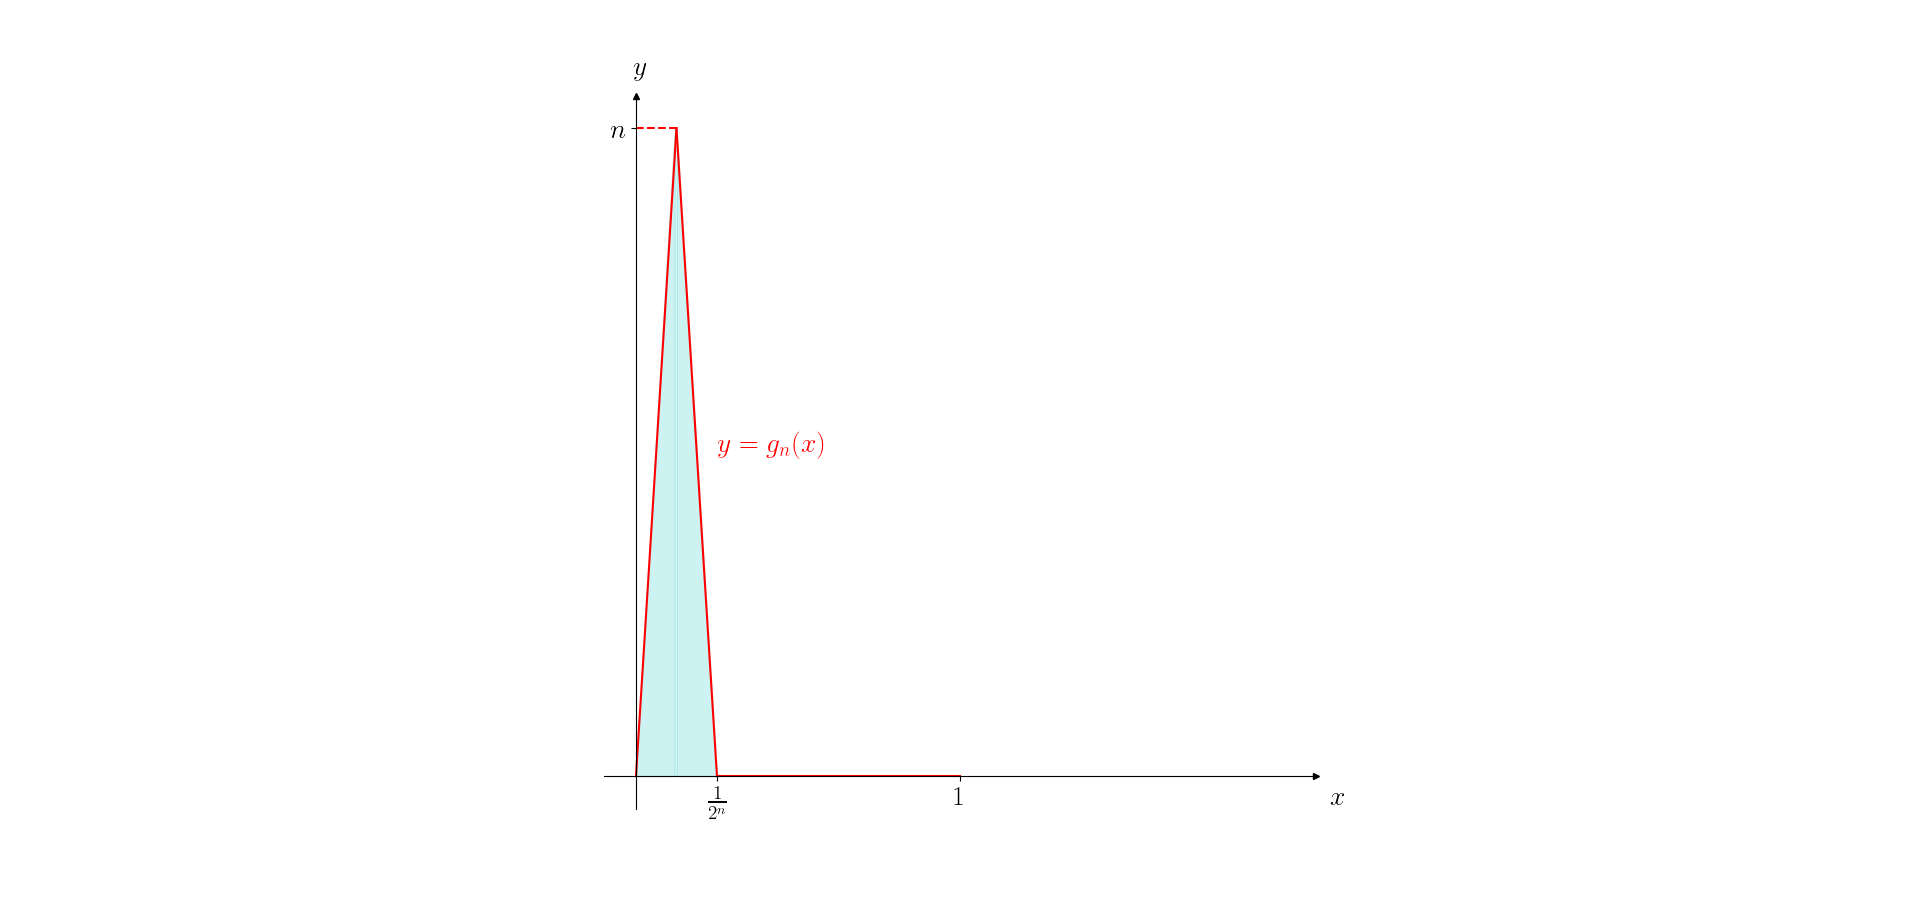
\includegraphics[width=0.85\linewidth]{spazi_metrici_e_normati/pag139triangolo}
	\end{center}

	$\int_{0}^{1} |g_n(x)| \ \mathrm{d}x =$ area del triangolo $ = \frac{1}{2} \frac{1}{2^n} n = \lowercomment{\frac{n}{2^{n+1}}} {\myarrow[270]} {0 \text{ per } n \rightarrow + \infty}$

	Fissato $r > 0$, trovo $n$ tale che $\int_{0}^{1} |g_n(x)| \ \mathrm{d}x < r$	
\end{exbar}


\begin{definition}
	$x \in X$. Un \textbf{intorno di $x$} è un qualsiasi sottoinsieme $A \subseteq X$ che contiene una palla aperta centrata in $x$, cioè per cui $\exists \ r > 0 \big| B_r(x) \subseteq A$
\end{definition}


\begin{definition}
	$A \subseteq X$ si dice \textbf{aperto} se è intorno di ogni suo punto, cioè se $\forall \ x \in A \quad \exists r > 0 \ \big| \ B_r(x) \subseteq A$.
	
	$A$ si dice \textbf{chiuso} se $A^c = X \backslash A$ è aperto.
\end{definition}


\begin{exbar}
\begin{example}
	$(x,d)$ spazio metrico, $x \in X, r>0$, $B_r(x)$ è un aperto.
	
	Devo far vedere che $\forall \ y \in B_r(x) \ \exists \ \overline{r} > 0 \ \big| \; B_{\overline{r}}(y) \subseteq B_r(x)$
	
	$\overline{r} = r - d(x,y) > 0$ perché $d(x,y) < r$ e dimostriamo che, se $z \in B_{\overline{r}} (y)$, allora $z\in B_r(x)$, cioè, se $d(y,z)< \overline{r}$, allora $d(x,z)<r$
	
	$d(x,z) \distr  d(x,y) + d(y,z) < d(x,y) + \overline{r} = d(x,y) + (r-d(x,y)) = r$	
	\begin{center}
		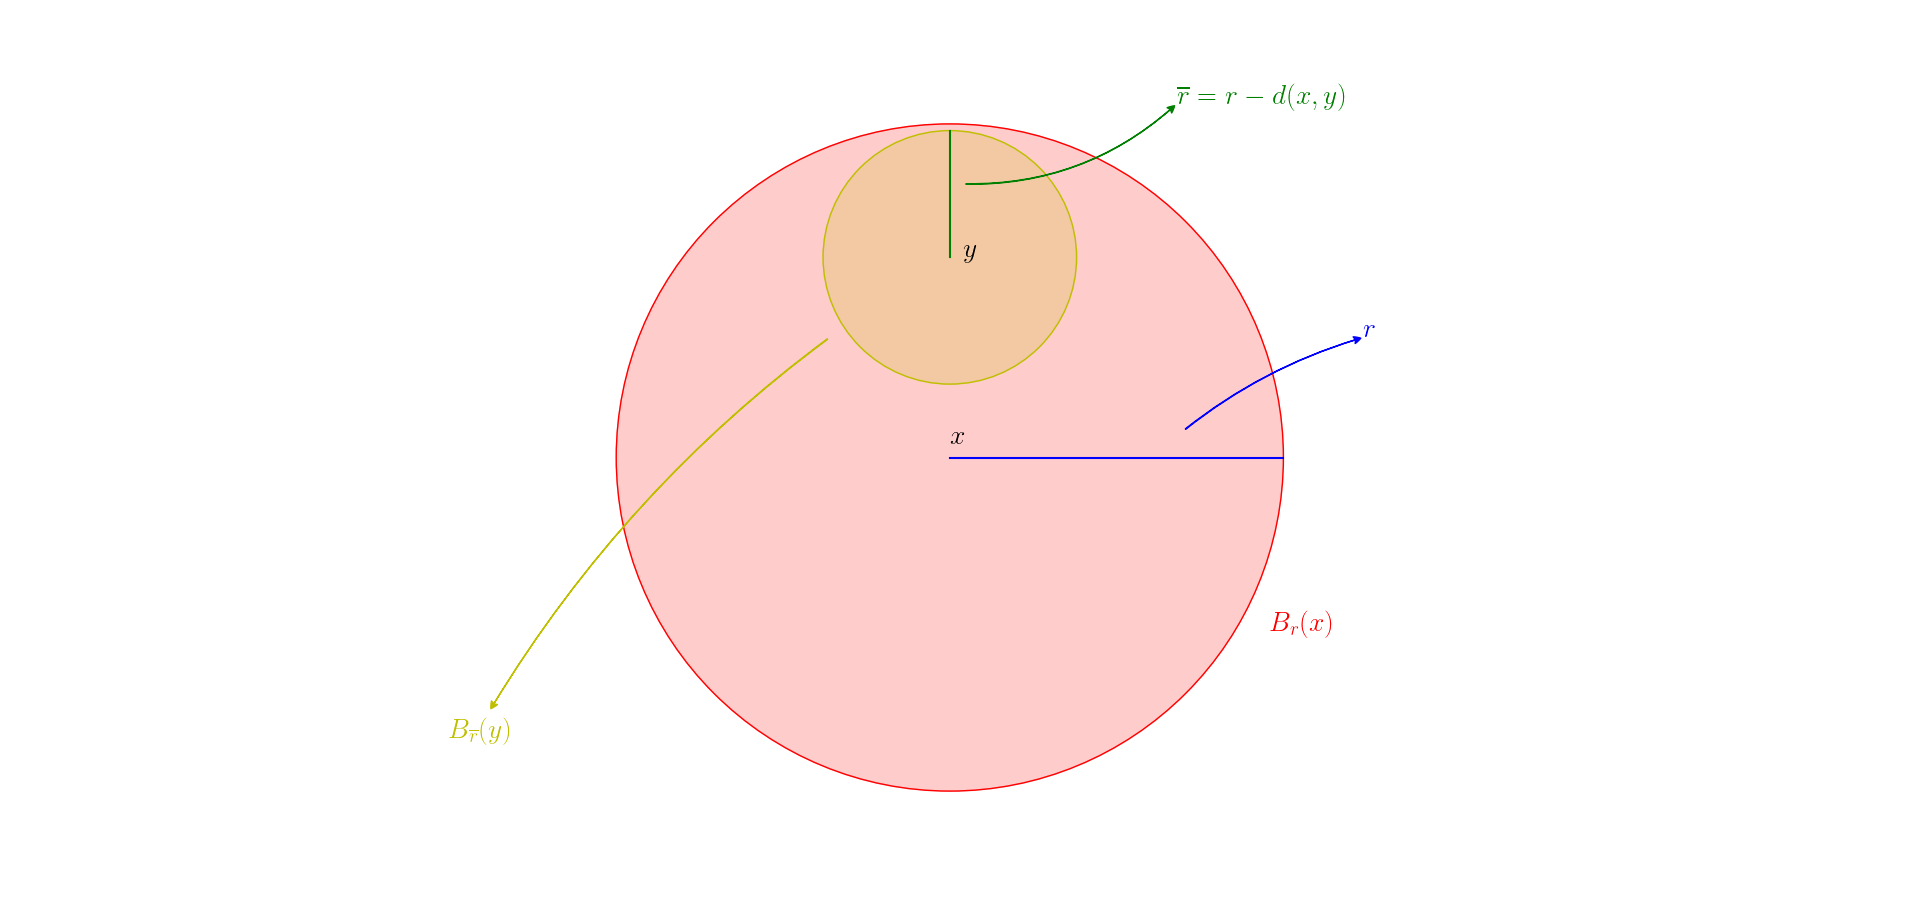
\includegraphics[width=0.75\linewidth]{spazi_metrici_e_normati/pag141}
		\label{fig:pag141}
	\end{center}
\end{example}
\end{exbar}


\begin{exbar}
	$(\mathbb{R}^2, \parallel \cdot \parallel_\infty)$
	\begin{center}
		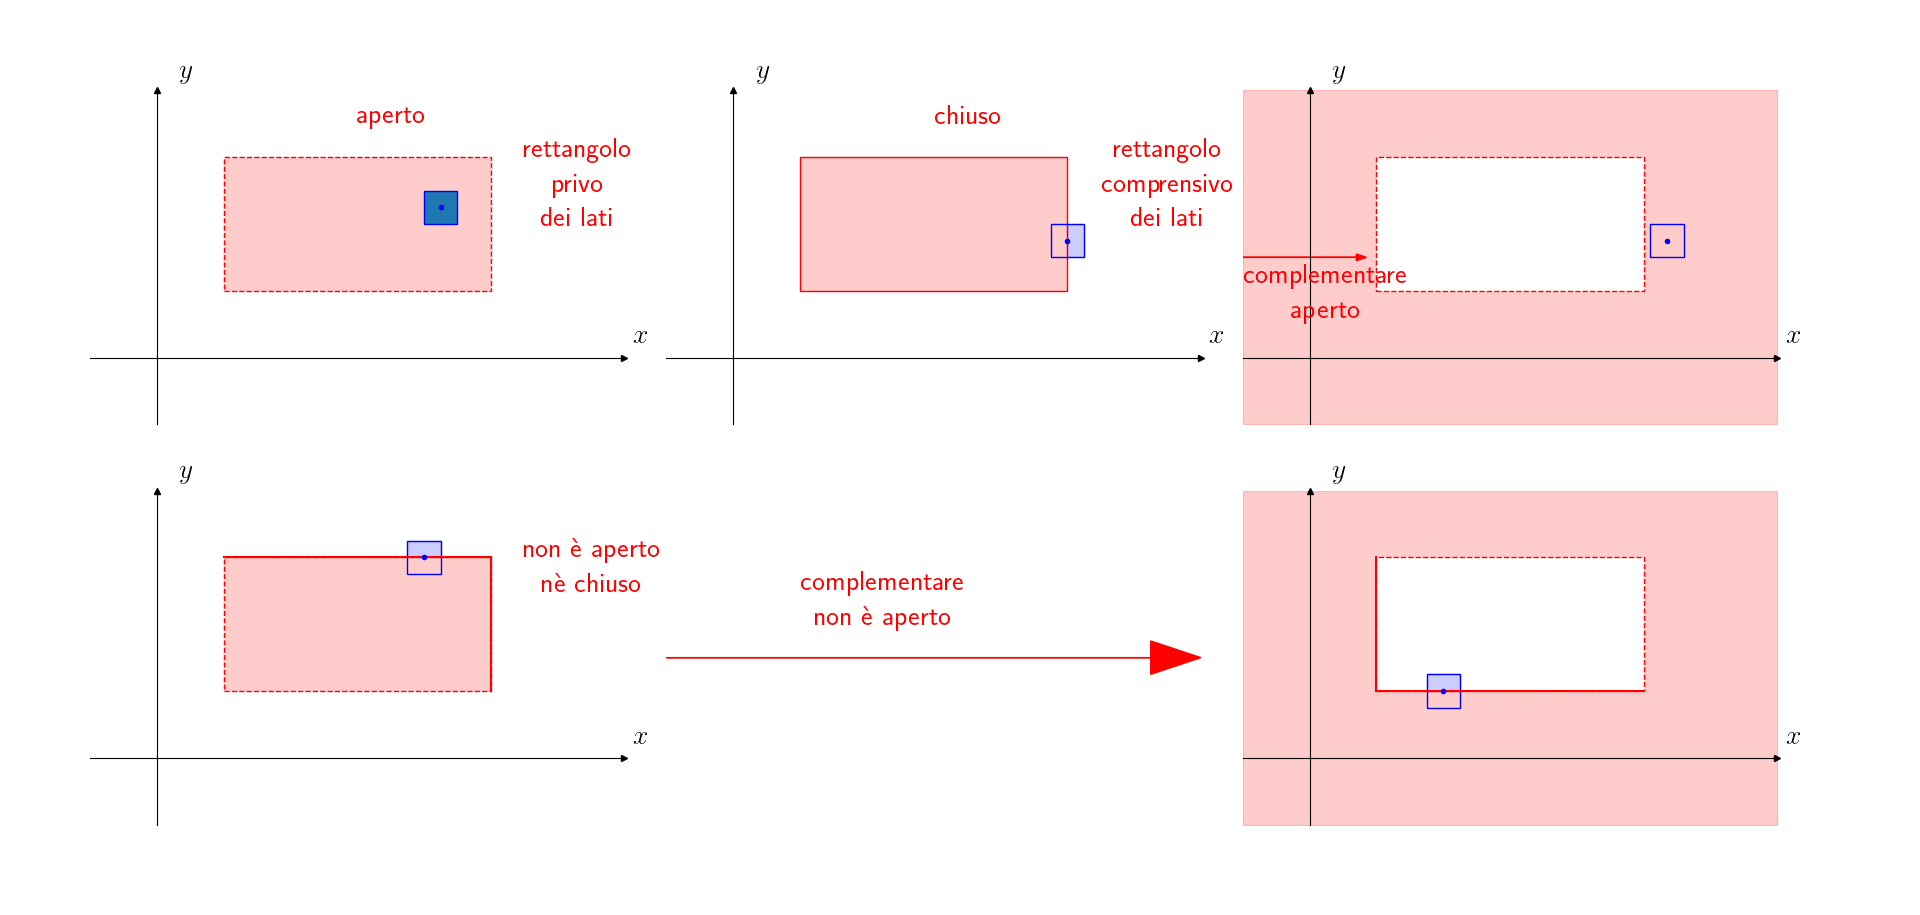
\includegraphics[width=\linewidth]{spazi_metrici_e_normati/pag141-142}
		\label{fig:pag141-142}
	\end{center}
\end{exbar}


\textbf{Osservazione:} 
	$(X,d)$ spazio metrico, $X$ è aperto banalmente (se $x \in X, B_r(x) \subseteq X \ \forall \ r > 0$) e quindi $\emptyset = X^c = X \backslash X$ è chiuso. 
	
	D'altra parte $\emptyset $ è aperto perché l'implicazione $x \in \emptyset \Rightarrow  \ \exists \ r > 0 \ \big| \ B_r(x) \subseteq \emptyset$ è vera perché $x \in \emptyset$  è falsa $\Rightarrow \emptyset^c = X \backslash \emptyset = X$ è chiuso. 
	
	\begin{attbar}
		$\emptyset, X$ sono sia aperti che chiusi.
	\end{attbar}


\begin{theorem}
	
	$(X,d)$ spazio metrico
	\begin{enumerate}
		\item $A_1, A_2 \subseteq X$ aperti $\Rightarrow A_1 \cap A_2$ è un aperto.
		 
		\item $\{A_i\}_{i \in I}$ è una famiglia di aperti, allora $\bigcup_{i \in I} A_i$ è un aperto.
		
		\item Se $C_1, C_2 \subseteq X$ sono chiusi, allora $C_1 \cup C_2$ è chiuso.
		
		\item $\{C_i\}_{i\in I}$ è famiglia di chiusi, allora $\bigcap_{i \in I} C_i$ è un chiuso.
	\end{enumerate}
\end{theorem}


\textbf{Osservazione:} 
In generale se $\{ A_i \}_{i \in I}$ è una famiglia infinita di aperti, allora $\bigcap_{i \in I} A_i$ non è un aperto e, se $\{ C_i \}_{i \in I}$ è una famiglia infinita di chiusi, allora $\bigcup_{i \in I} C_i$ non è chiuso. Facciamo un esempio.

$A_k= \ \bigg]-\frac{1}{k}, \frac{1}{k} \bigg[ \qquad k \geq 1, k \in \mathbb{N}$ sono tutti aperti di $\mathbb{R}$, allora $\bigcap_{k=1}^\infty A_k = \bigcap_{k=1}^\infty \ \bigg] -\frac{1}{k}, \frac{1}{k} \bigg[ \ = \{ 0 \}$, che è un chiuso.

$C_k = \left[ \frac{1}{k}, 1-\frac{1}{k} \right], \qquad k \geq 2, k \in \mathbb{N}$ sono tutti chiusi 

\bigg( $C_k^c = \ \bigg] -\infty, \frac{1}{k} \bigg[ \ \cup \ \bigg] 1-\frac{1}{k}, +\infty \bigg[$, unione di due intervalli aperti \bigg)

$\bigcup_{k=2}^\infty C_k = \bigcup_{k=2}^\infty \left[ \frac{1}{k}, 1-\frac{1}{k} \right] = \ ]0,1[$

Infatti, se $x \in \bigcup_{k=1}^\infty \left[ \frac{1}{k}, 1-\frac{1}{k} \right]$, allora $\exists \ \overline{k} \geq 2 \ \big| \ \left[\frac{1}{k}, 1-\frac{1}{k}\right]$, cioè $0 < \frac{1}{k} \leq x \leq 1- \frac{1}{k} < 1$

$\Rightarrow 0 < x < 1 \Rightarrow x \in \ ]0,1[.$

D'altra parte, se $x \in \ ]0,1[$, esistono $k_1$ e $k_2 \ \big| \ \frac{1}{k_1} < x<1 - \frac{1}{k_2}$

$k=\max\{k_1, k_2\}$ 

\begin{gather*}
	\frac{1}{k} \leq \frac{1}{k_1} < x < 1 - \frac{1}{k_2} \leq 1 - \frac{1}{k}
	\\
	\Rightarrow x \in C_k = \left[ \frac{1}{k}, 1 - \frac{1}{k} \right]
	\\
	\Rightarrow x \in \bigcup_{k=2}^{\infty} C_k
\end{gather*}


\begin{definition}
	
	$(X,d)$ spazio metrico, $A \subseteq X, \ x \in A$. $x$ si dice \textbf{punto interno di A} se $\exists \ r > 0 \ \big| \ B_r(x) \subseteq A$. L'interno di $A$ è l'insieme dei punti interni di $A$ ed è indicato con \AA
\end{definition}


\begin{proposition}
	\label{pr: grande aperto}
	\AA \ è un insieme aperto ed è il più grande aperto, nel senso dell'inclusione, contenuto in $A$, cioè se $B \subseteq A$ è aperto, allora $B \subseteq \AA$
\end{proposition}

\begin{dembar}
	\textbf{Dimostrazione} della \textbf{Proposizione \ref{pr: grande aperto}} (Esercizio per casa)
\end{dembar}


\begin{exbar}
	\begin{gather*}
		A = \ ]0,1], \qquad \AA = \ ]0,1[
		\\
		A = \ ]0,1] \cup \{ 2 \}, \qquad \AA = \ ]0,1[
		\\
		A = \ ]0,1] \cup \left\{2 + \frac{1}{n} \ \bigg| \ n \geq 1, n \in \mathbb{N} \right\}, \qquad \AA = \ ]0,1[
	\end{gather*}
\end{exbar}


\begin{definition}
	$A \subseteq X, x \in X$ si dice \textbf{punto di chiusura} per $A$ se $B_r(x) \cap A \neq \emptyset \ \forall \ r > 0$, cioè ogni palla di centro $x$ interseca $A$. 
	
	La chiusura di $A$ è l'insieme di tutti i punti di chiusura di $A$ ed è denotata con $\overline{A}$.
\end{definition}


\begin{proposition}
	\label{pr: grande chiuso}
	$\overline{A} $ è un insieme chiuso ed è il più piccolo chiuso, nel senso dell'inclusione, contenente $A$, cioè, se $C \geq A$ è chiuso, allora $\overline{A} \subseteq C$
\end{proposition}


\begin{dembar}
	\textbf{Dimostrazione} della \textbf{Proposizione \ref{pr: grande chiuso}} (Esercizio per casa)
\end{dembar}


\begin{exbar}
	\begin{gather*}
		A = \ ]0,1], \qquad \lowercomment{\overline{A} = [0,1]} {0 \notin A, \text{ mentre se } x \in \AA \Rightarrow x \in A} {x \in A \Rightarrow x \in \overline{A} \text{ perché } x \in B_r(x) \cap A \ \forall r > 0}
		\\
		A = \ ]0,1] \cup \{ 2 \}, \qquad \overline{A} = [0,1] \cup \{ 2 \}
		\\
		A = \ ]0,1] \cup \left\{ 2 + \frac{1}{n} \ \bigg| \ n \geq 1, n \in \mathbb{N} \right\}, \qquad \overline{A} = [0,1] \cup \left\{2 + \frac{1}{n} \ \bigg| \ n \geq 1, n \in \mathbb{N} \right\} \cup \{ 2 \}	\end{gather*}
\end{exbar}


\textbf{Osservazione:}
\begin{gather*}
	\AA \subseteq A \subseteq \overline{A}
	\\	
	A \text{ è aperto } \iff A = \AA
	\\
	A \text{ è chiuso } \iff A = \overline{A}
\end{gather*}

$(\Leftarrow) A=\overline{A}$, $\overline{A}$ è un chiuso $\Rightarrow A$ è chiuso

$(\Rightarrow)$ Sia $A$ chiuso e dimostriamo che $A = \overline{A}$. Noi sappiamo che $A \subseteq \overline{A}$.

Se per assurdo $A \nsubseteq \overline{A}, \; \exists \ x \in \overline{A} \ \big| \ x \notin A$, cioè $x \in \overline{A}$ e $x \in A^c$. Ma $ A^c $ è aperto, perché $ A $ è chiuso, e quindi $ \exists r > 0 \ \big| \ B_r (x) \subseteq A^c$

$\Rightarrow B_r (x) \cap A = \emptyset$, assurdo perché $x \in \overline{A}$.


\begin{definition}
	$A \subseteq X, x \in X$ si dice \textbf{punto di frontiera} per $A$ se $\forall \ r > 0 \quad B_r(x) \cap A \neq \emptyset$ e $B_r(x) \cap A^c \neq \emptyset$, cioè se ogni palla di centro $x$ interseca sia $A$ che il suo complementare.
	
	L'insieme dei punti di frontiera di $A$ si dice frontiera di $A$ e si indica con $\partial A$. 
\end{definition}


\begin{exbar}
	\begin{gather*}
		A = ]0,1], \qquad \partial A = \{0,1\} 
		\\
		A = \ ]0,1] \cup \{ 2 \}, \qquad \partial A = \{ 0, 1, 2 \}
		\\
		A = \ ]0,1] \cup \left\{ 2 + \frac{1}{n} \ \bigg| \ n \geq 1, n \in \mathbb{N} \right\}, \qquad \partial A = \{0,1\} \cup \left\{2 + \frac{1}{n} \ \bigg| \ n \geq 1, n \in \mathbb{N} \right\} \cup \{ 2 \}
	\end{gather*}
$(\mathbb{R}^2, \parallel \cdot \parallel_\infty)$
g
\begin{center}
	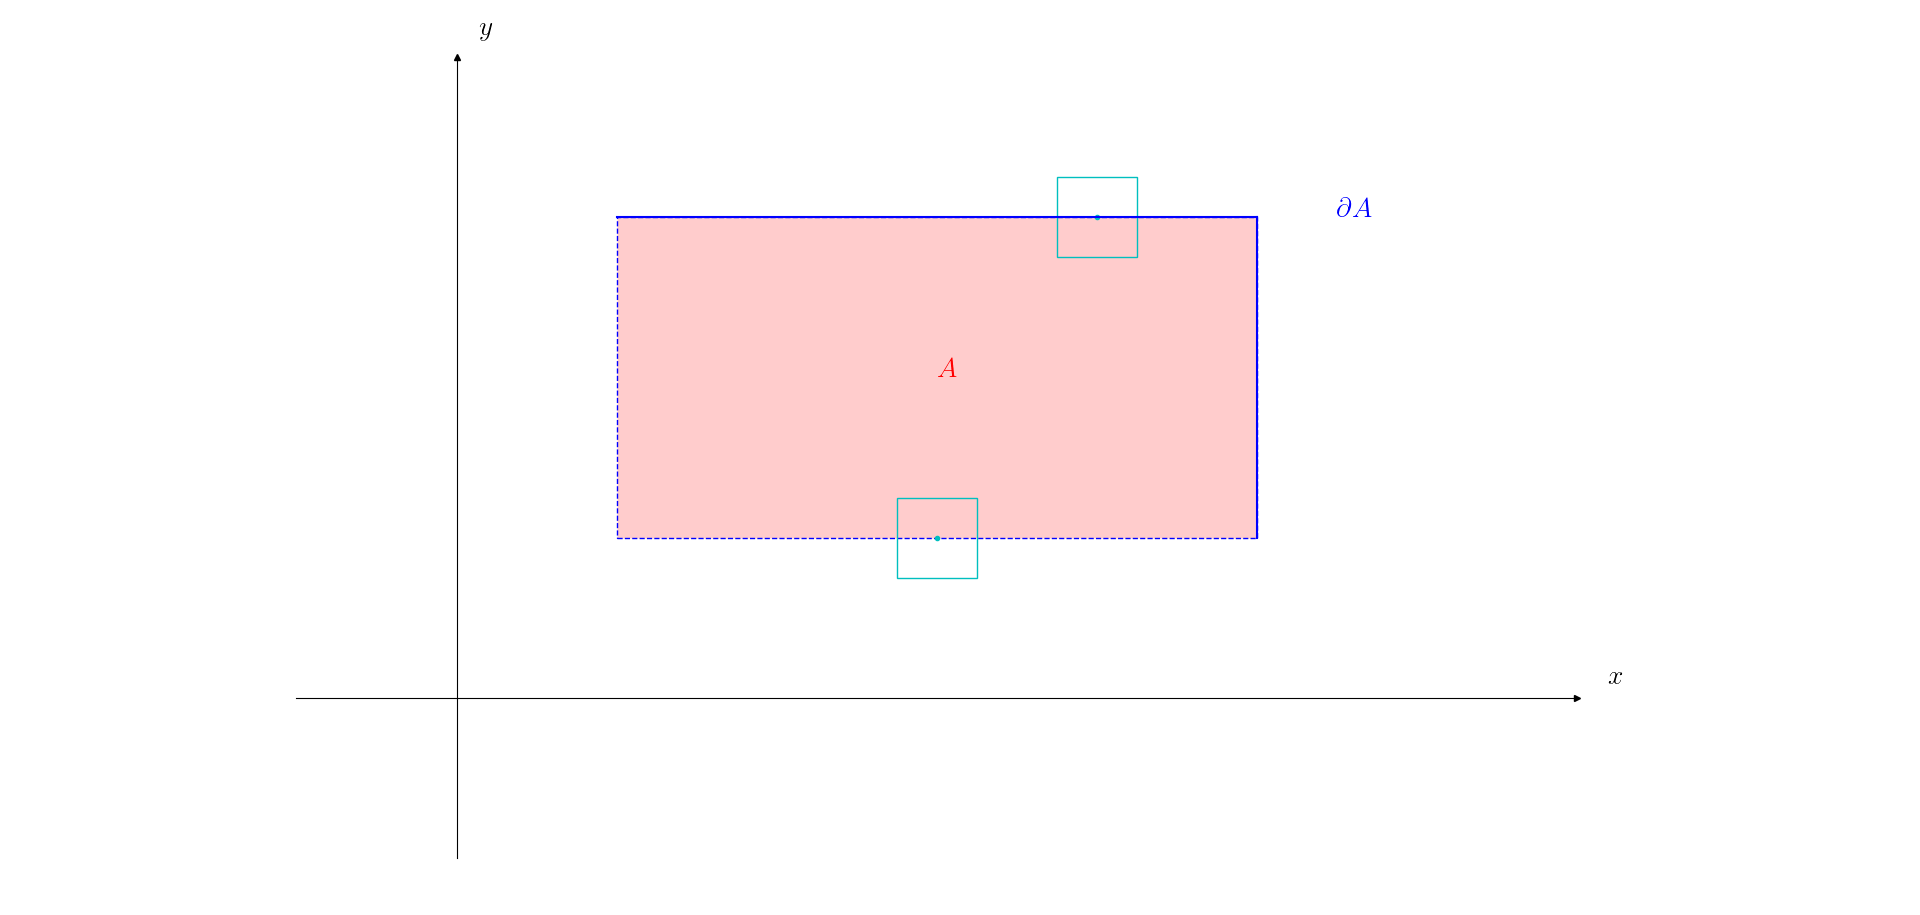
\includegraphics[width=0.65\linewidth]{spazi_metrici_e_normati/pag148}
	\label{fig:pag148}
\end{center}
\end{exbar}


\textbf{Osservazione:}

\begin{itemize}
\item $\partial A = \overline{A} \cap \overline{A^c}$
\begin{gather*}
	x \in \partial A \Rightarrow B_r (x) \cap A \neq \emptyset \qquad \forall \ r > 0, \; x \in \overline{A}
	\\
	\Rightarrow B_r(x) \cap A^c \neq \emptyset \qquad \forall r > 0, \; x \in \overline{A^c}
	\\
	\Rightarrow x \in \overline{A} \cap \overline{A^c} \Rightarrow \partial A \subseteq \overline{A} \cap \overline{A^c}
	\\
	x \in \overline{A} \cap \overline{A^c} \Rightarrow x \in \overline{A} \text{ e } x \in \overline{A^c}
	\\
	\begin{array}{c c}
		x \in \overline{A} \Rightarrow B_r(x) \cap A \neq \emptyset \quad \forall \ r > 0
		\\
		x \in \overline{A^c} \Rightarrow B_r(x)\cap A^c \neq \emptyset \quad \forall \ r > 0
	\end{array}
	\Rightarrow x \in \partial A
	\\
	\Rightarrow \overline{A} \cap \overline{A^c} \subseteq \partial A
\end{gather*}

\item $\overline{A}=A \cup \partial A$

\begin{equation*}
	A \subseteq \overline{A}, \; \partial A \subseteq \overline{A} \Rightarrow A \cup \partial A \subseteq \overline{A}
\end{equation*}
Facciamo vedere che $\overline{A} \subseteq A \cup \partial A$.
	
$x \in \overline{A}$, supponiamo che $x \notin A$ e dimostriamo che $x \in \partial A$
	
\begin{gather*}
	x \in \overline{A}  \Rightarrow \lowercomment{B_r(x) \cap A \neq \emptyset} {(x \notin A \Rightarrow x \in A^c)} {} \qquad \forall \ r > 0
	\\
	x \in B_r (x) \cap A^c \qquad \forall \ r > 0
	\\
	\mathcircled{B_r(x) \cap A^c \neq \emptyset \qquad \forall \ r > 0}
	\\
	\Rightarrow x \in \partial A, \text{ come si voleva}
\end{gather*}
\end{itemize}


\begin{attbar}
	$A$ è chiuso $\iff \partial A \subseteq A$, cioè se e solo se $A$ contiene la sua frontiera.
\end{attbar}


\begin{exbar}
\begin{example}
	$(\mathbb{R}, |\cdot|), \qquad \mathbb{Q} \subseteq \mathbb{R}$
	
	\begin{gather*}
		\overline{\mathbb{Q}} = \mathbb{R}
		\\
		\text{Fissati } x\in \mathbb{R} \text{ e }  r > 0 \quad \exists \ q \in \mathrm{Q} \text{ tale che }  q \in \ ]x-r, x+r[ \ = B_r(x)
		\\
		\partial \mathbb{Q} = \mathbb{R}
		\\
		x \in \mathbb{R}, \ B_r(x) \cap \mathbb{Q} \neq \emptyset \qquad \forall \ r > 0, B_r(x) \cap \ \mathbb{Q}^c \neq \emptyset \qquad \forall \ r > 0
		\\
		]x-r,x+r[ \ \cap \mathbb{Q}^c \neq \emptyset \qquad \forall \ r > 0
	\end{gather*}
	
	Se non fosse vero, $\exists \ x \in \mathbb{R}$ e $r > 0$ tale che $]x-r, x+r[$ è fatto tutto di numeri razionali.
	
	I razionali sono numerabili, cioè $\exists f: \mathbb{N} \rightarrow \mathbb{Q} $ iniettiva e suriettiva. I reali hanno la potenza del continuo, cioè ogni funzione $\phi: \mathbb{N} \rightarrow \mathbb{R}$ può essere al più iniettiva, ma non suriettiva. Questo è vero anche per ogni intervallo del tipo $]x-r, x+r[, r > 0$. Quindi, se $]x-r, x+r[$ fosse fatto di soli numeri razionali, sarebbe numerabile, assurdo.
\end{example}
\end{exbar}


\subsection{Successioni in spazi metrici}
\begin{exbar}
\begin{itemize}
	\item $\mathbb{R}^2 \qquad \{(e^{-n}, \frac{\sin n}{n}) \}_{n\geq 1}$ è una successione di elementi di $\mathbb{R}^2$
	\item $\mathbb{R}^3 \qquad \{ (1+\frac{1}{n}, \frac{\sinh n}{e^n},2^{-n}) \}$ è una successione di elementi di $\mathbb{R}^3$
\end{itemize}
\end{exbar}


\begin{definition}
	$\{x_k\}_{k\in \mathbb{N}} \subseteq X$ successione, con $(X,d)$ spazio metrico. 
	
	Si dice che $\{ x_k\}_{k \in \mathbb{N}}$ converge ad $x \in X$ e si scrive
	\begin{equation*}
		x_k \rightarrow x \qquad \text{o} \qquad \lim_{k\rightarrow +\infty} x_k = x \iff \lim_{k \rightarrow +\infty} d(x_k, x) = 0
	\end{equation*}
	
	(in ambito reale $\lim_{k \rightarrow +\infty} |x_k - x |=0$)
	
	cioè $\iff \forall \ \epsilon > 0 \ \exists \ N > 0 \ \big| \ k > N$
	
	$\Rightarrow d(x_k,x) < \epsilon$
	
	$x$ viene detto \textbf{limite della successione}.
	
\end{definition}


\begin{theorem}
	Sia $\{ x_k \}_{k \in \mathbb{N}} \subseteq X, (X,d)$ spazio metrico, tale che 
	\begin{equation*}
		x_k \rightarrow l_1 \in X \text{ e } x_k \rightarrow l_2 \in X
	\end{equation*}
	
	Allora $l_1=l_2$.
\end{theorem}


\begin{proposition}
	\label{pr:pag152}
	$\{\overline{x_k}\}_{k \in \mathbb{N}} \subseteq R^n$ tale che $\overline{x_k } = (x_{k_1}, x_{k_2}, \ldots, x_{k_n})$. Allora
	\begin{equation*}
		\overline{x_k} \rightarrow \overline{x} = (x_1, \ldots, x_n) \iff x_{k_{j}} \rightarrow x_{j} \qquad \forall \ j = 1, \ldots, n
	\end{equation*}
	
	cioè $\iff \forall \ j = 1, \ldots, n$ la successione di numeri reali $\{ x_{kj} \}_{k \in \mathbb{N}}$ converge a $x_{j}$.
\end{proposition}


\begin{exbar}

\begin{itemize}
	\item $\mathbb{R}^2, \left\{ \underbrace{ \left(e^{-k}, \frac{\sin k}{k} \right)} _ {\overline{x_k}} \right\}_{k \geq 1}$
	\begin{gather*}
		\overline{x_k} = (x_{k_1}, x_{k_2})
		\\
		\begin{array}{c c}
			x_{k_1} = e^{-k}, &
			x_{k_2} = \frac{\sin k}{k}
			\\
			\lim_{k \rightarrow +\infty} x_{k_1}=0, & \lim_{k \rightarrow +\infty} x_{k_2} = 0
		\end{array}
		\\
		\Rightarrow \lim_{k \rightarrow + \infty} \overline{x_k} = (0,0)
	\end{gather*}
	
	\item $\mathbb{R}^3, \left\{ \underbrace{ \left(1 + \frac{1}{k}, \frac{\sinh k}{e^k}, 2^{-k} \right)} _ {\overline{x_k}} \right\}_{k \geq 1}$
	\begin{gather*}
		\begin{array}{c c c}
		x_{k_1} = 1 + \frac{1}{k}, 
		& x_{k_2} = \frac{\sinh k}{e^k}, 
		& x_{k_3} = 2^{-k}
		\\
		\lim_{k \rightarrow +\infty} x_{k_1} = 1, \quad
		& \lim_{k \rightarrow +\infty} x_{k_2} = 1, \quad 
		& \lim_{k \rightarrow +\infty} x_{k_3} = 0 
	\end{array}
		\\
		\lim_{k \rightarrow +\infty} \overline{x_k} = (1, 1, 0)
	\end{gather*}

	\item $\mathbb{R}^2, \left\{ \underbrace{(2+e^{-k}, \sin k)} _ {\overline{x_k}} \right\} $
	\begin{gather*}
	\begin{array}{c c}
		x_{k1} = 2+e^{-k}, \quad 
		& x_{k2} = \sin k
		\\
		\lim_{k \rightarrow +\infty} x_{k_1} = 2, \quad 
		& \lim_{k \rightarrow +\infty} \nexists
	\end{array}
		\\
		\Rightarrow \lim_{k \rightarrow +\infty} \overline{x_k} \nexists
	\end{gather*}

\end{itemize}
\end{exbar}


\begin{dembar}
	\textbf{Dimostrazione} della \textbf{Proposizione \ref{pr:pag152}}
	
	
	$(\mathbb{R}^n, |\cdot|)$
	
	Se $\overline{y} = (y_1, \ldots, y_n) \in \mathbb{R}^n$, allora 
	\begin{gather*}
		|y_j| \leq |\overline{y}| \leq \sum_{i=1}^{n} |y_i| \qquad \forall \ j
		\\
		|y_j| = \sqrt{|y_j|^2} \leq \sqrt{\sum_{i=1}^{n} |y_i|^2} = |\overline{y}|
	\end{gather*}
	
	Abbiamo dimostrato che, se $0 < p < 1$, 
	\begin{equation*}
		(a+b)^p \leq a^p + b^p \qquad \forall \ a,b \geq 0
	\end{equation*}
	
	Questa disuguaglianza si può generalizzare.
	\begin{gather*}
		(a_1 + a_2 + \ldots + a_n)^p \leq a_1^p + a_2^p + \ldots + a_n^p \qquad \forall \ a_i \geq 0
		\\
		|\overline{y}| = \sqrt{\sum_{i=1}^{n} |y_i|^2} 
		\uppercomment{\leq} {p=\frac{1}{2}} {a_i = (y_1)^2} 
		(|y_1|^2)^{1/2} + (|y_2|^2)^{1/2} + \ldots + (|y_n|^2)^{1/2} =
		\\
		= |y_1| + |y_2| + \ldots + |y_n| = \sum_{i=1}^{n} |y_i|
		\\
		\uppercomment{|y_j|} {} {y_j = x_{k_{j}} - x_j}
		\leq |\overline{y}| \leq \sum_{i=1}^{n} |y_i|
		\\
		\overline{x_k} \rightarrow \overline{x} \iff x_{k_j} \rightarrow x_j \qquad \forall \, j = 1, \ldots, n
		\\
		|x_{k_{j}} - x_j| \leq |\overline{x_k} - \overline{x}| \leq \sum_{i=1}^{n} |x_{k_i} - x_i|
	\end{gather*}

	Se $|\overline{x_k} - \overline{x}| \rightarrow 0 $, cioè se $\overline{x_k} \rightarrow \overline{x}$, allora
	\begin{equation*}
		0 \leq \lowercomment{|x_{kj}-x_j|} {\myarrow[270]} {0 \text{ per confronto}} \leq |\overline{x_k} - \overline{x}| \Rightarrow x_{k_{j}} \rightarrow x_j \qquad \forall \ j
	\end{equation*}
	
	D'altra parte, se $x_{k_{i}} \rightarrow  x_i \quad \forall \ i = 1, \ldots, n$
	\begin{gather*}
		\Rightarrow \sum_{i=1}^{n} |x_{k_i} - x_i| \rightarrow 0 \text{ per } k \rightarrow + \infty
		\\
		\Rightarrow 0 \leq |x_{k} - x| \leq \sum_{i=1}^{n} |x_{k_{i}} - x_i| \Rightarrow \overline{x_k} \rightarrow \overline{x} \qquad \square
	\end{gather*}	
\end{dembar}


\begin{theorem} (caratterizzazione dei chiusi mediante le successioni)
\label{th:pag 156}	
	
$(X,d)$ spazio metrico, $A \subseteq X$. Allora $z \in \overline{A} \iff \exists$ una successione $\{x_k\}_{k \geq 1} \subseteq A \ \big| \ x_k \rightarrow z$.
\end{theorem}


\begin{corollary}
	\label{cor:pag 156}
	$(X,d)$ spazio metrico. $A \subseteq X$ è chiuso $\iff \forall \ \{x_k\}_{k \geq 1} \subseteq A$ convergente, il suo limite appartiene ad $A$.
	
	($A \subseteq X$ è chiuso $\iff A$ contiene i limiti delle successioni convergenti a valori in $A$.)
\end{corollary}


\begin{dembar}
	\textbf{Dimostrazione} del \textbf{Corollario \ref{cor:pag 156}}
	
	\begin{itemize}
		\item $(\Rightarrow) \ A$ chiuso, $A = \overline{A}$. Sia $\{x_k\}_{k \geq 1} \subseteq A$ successione convergente a $z \in X$.
		
		Allora il teorema implica che $z \in \overline{A}= A$.
		
		\item $(\Leftarrow)$ Dobbiamo dimostrare che, se $x \in \overline{A}$, allora $z \in A$
		
		($A = \overline{A}$, perché l'inclusione $A \subseteq \overline{A}$ è nota)
		
		$z \in \overline{A} \Rightarrow \exists \ \{x_k\}_{k \geq 1} \subseteq A$ convergente a $z$. 
		
		Allora $z \in A$ per ipotesi. $\qquad \square$
	\end{itemize}
\end{dembar}


\begin{dembar}
	\textbf{Dimostrazione} del \textbf{Teorema \ref{th:pag 156}}
	
	\begin{itemize}
		\item $(\Rightarrow ) $ Sia $z \in \overline{A}$. Costruiamo una successione $\{x_k\}_{k \geq 1} \subseteq A \ \big| \ x_k \rightarrow z$
		\begin{gather*}
		z\in \overline{A} \iff \forall \ r > 0, B_r(z) \cap A \neq \emptyset
		\\
		\begin{array}{c c}
			r = 1 
			& \exists \ x_1 \in B_1(z) \cap A 
			\\ & x_1 \in A \text{ e } d(x_1, z) < 1
			\\
			r = \frac{1}{2}
			& \exists \ x_2 \in B_{1/2}(z) \cap A
			\\ & x_2 \in A \text{ e } d(x_2, z )< \frac{1}{2}
			\\
			\vdots & \\
			r=\frac{1}{k}
			& \exists \ x_k \in B_{\frac{1}{k}}(z) \cap A,
			\\ & x_k \in A \text{ e } d(x_k, z) < \frac{1}{k}
		\end{array}
		\\
		\{x_k\}_{k \geq 1} \subseteq A \ \big| \; 0 \leq d(x_k, z) \leq \frac{1}{k} 
		\\ \Rightarrow \lim_{k \rightarrow +\infty} d(x_k, z) = 0 \Rightarrow x_k \rightarrow z
		\end{gather*}
		
		\item $()\Leftarrow )$ Ipotesi: $\exists \ \{x_k\}_{k\geq 1} \subseteq A \ \big| \ x_k \rightarrow z$
		
		Tesi: $z \in \overline{A}$
		
		Sia $r >0$. Poiché $x_k \rightarrow z$
		\begin{gather*}
		\exists \ N > 0 \ \big| \; d(x_k,z) < r \qquad \forall \ k > N, \lowercomment{x_k} {\in A} {} \in B_r(z) \cap A
		\\
		\Rightarrow B_r(z) \cap A \neq \emptyset \Rightarrow z \in \overline{A}. \qquad \square
		\end{gather*} 
	\end{itemize}
\end{dembar}







\begin{comment}	



\paragraph{\textcolor{red}{Esempi}}
\begin{itemize}
	\item $\Q$ non è chiuso in  $\R$ perchè $\exists \,\, \{q_n\}_{n\geq 1} \subseteq \Q \,\,|\,\, q_n \rightarrow \sqrt{2} \neq \Q$
	\item $(\R, |\cdot|)$
\end{itemize}
\begin{figure}[!h]
	\centering
	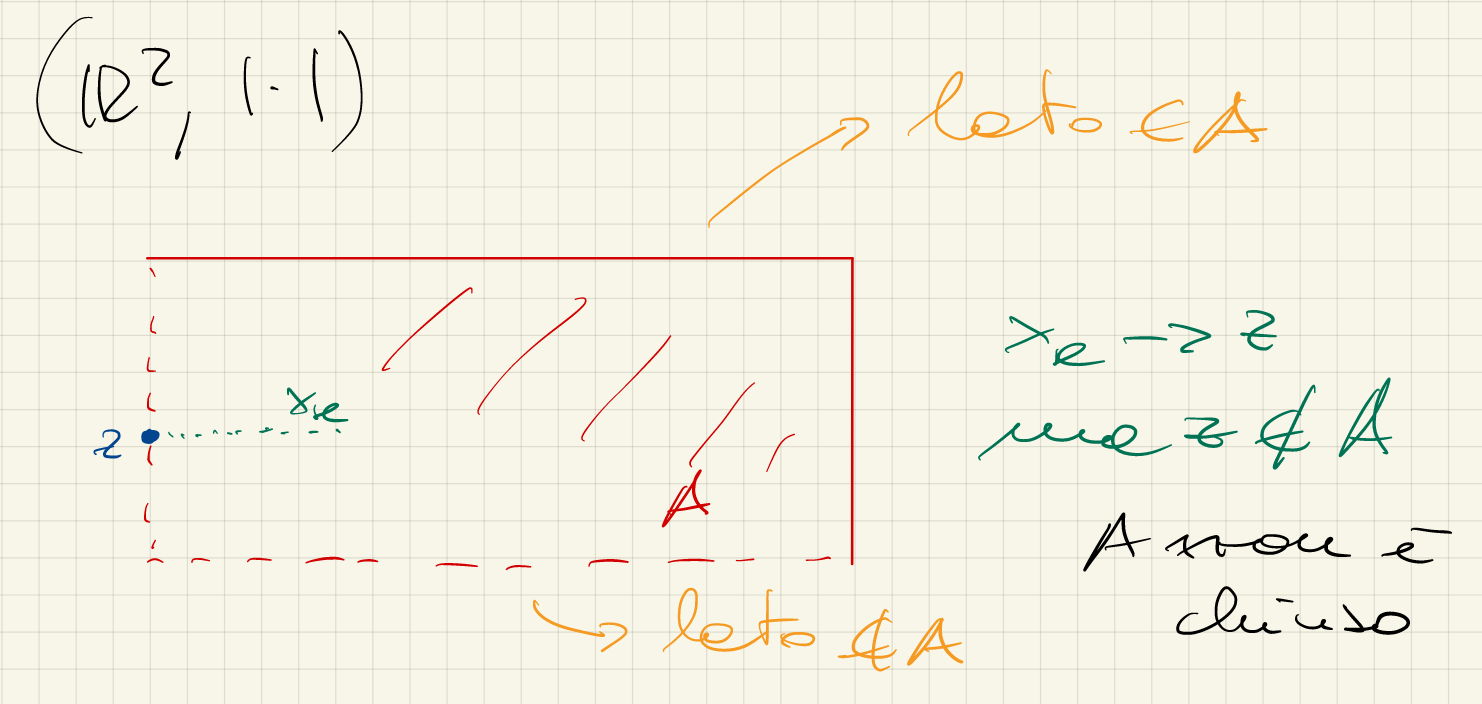
\includegraphics[width=0.5\textwidth]{Screenshot from 2023-03-28 18-09-08}
\end{figure}

\paragraph{\textcolor{red}{Esempio importante}}
$C\subseteq \R^n$. Sono equivalenti le seguenti affermazioni
\begin{enumerate}
	\item $C$ è chiuso per la topologia data dalla norma euclidea $|\cdot|$
	\item $C$ è chiuso per la topologia data dalla norma $\parallel \cdot \parallel_\infty$
	\item $C$ è chiuso per la topologia data dalla norma $\parallel \cdot \parallel_1$
\end{enumerate}
Per dimostrare che le tre affermazioni sono equivalenti, partiamo da\\
$|x_j|\leq |\overline{x}| \leq \sum_{i=1}^{n}|x_i| \,\,\forall\,\, \overline{x}=(x_1,...,x_n)\in \R^n$\\
$\max_{j=1,...,n}|x_j| \leq |\overline{x}| \leq \sum_{i=1}^{n}|x_i| \leq n \max_{j=1,...,n}|x_j|$\\
\textcolor{red}{$\parallel \overline{x} \parallel_\infty \leq |\overline{x}| \leq \parallel \overline{x} \parallel_1 \leq n \parallel \overline{x} \parallel_\infty \forall\,\, \overline{x} \in \R^n$}
\begin{itemize}
	\item $1) \Rightarrow 2)$ Ipotesi: $C$ è chiuso per $|\cdot|$. Tesi: $C$ è chiuso per $ \parallel \cdot \parallel_\infty$\\
	$\{\overline{x_k}\}_{k\geq 1} \subseteq C \,\, |\,\, \overline{x_k} \rightarrow \overline{z}$ per $\parallel \cdot \parallel_\infty$, cioè $\parallel \overline{x_k}-\overline{z} \parallel_\infty \rightarrow 0 $ per $k \rightarrow +\infty$, e dimostriamo che $\overline{z} \in C$\\
	$|\overline{x_k}-\overline{z}|\leq n \parallel \overline{x_k}-\overline{z} \parallel_\infty \rightarrow 0$\\
	$\Rightarrow |\overline{x_k}-\overline{z}| \rightarrow 0$ per $k \rightarrow +\infty$, cioè $\overline{x_k} \rightarrow \overline{z}$ per $|\cdot|$. Ma $C$ è chiuso per $|\cdot| \Rightarrow \overline{z} \in \C$.
	\item $2) \Rightarrow 3)$ Ipotesi: $C$ è chiuso per $\parallel \cdot \parallel_\infty$.        Tesi: $C$ è chiuso per $\parallel \cdot \parallel_1$\\
	$\{\overline{x_k}\}_{k \geq 1} \subseteq C \,\,|\,\, \overline{x_k} \rightarrow \overline{z}$ per $\parallel \cdot \parallel_1$, cioè $\parallel \overline{x_k}-\overline{z} \parallel_1 \rightarrow 0$ per $k \rightarrow +\infty$ e dimostriamo che $\overline{z}\in C$.\\
	$\parallel \overline{x} \parallel_\infty \leq \parallel \overline{x} \parallel_1 \,\, \forall \,\, \overline{x}\in \R^n$\\
	Prendo $\overline{x} = \overline{x_k} -\overline{z}$\\
	$\parallel \overline{x_k} -\overline{z} \parallel_\infty \leq  \parallel\overline{x_k} -\overline{z} \parallel_1 \rightarrow 0 \Rightarrow \overline{x_k}  \rightarrow \overline{z}$ per $\parallel \cdot \parallel_\infty \rightarrow \overline{z} \in \C$ perchè $C $ è chiuso  per $\parallel\cdot\parallel_\infty$.
	\item $3) \Rightarrow 1)$ Ipotesi: $C$ è chiuso per $\parallel \cdot \parallel_1$. Tesi:       $C$ è chiuso per $|\cdot|$\\
	$\{ \overline{x_k}\}_{k \geq 1} \subseteq C \,\, | \,\, \overline{x_k} \rightarrow \overline{z}$ per $|\cdot|$ e dimostriamo che $\overline{z} \in C$ \\
	$\parallel \overline{x} \parallel_1 \leq n \parallel \overline{x} \parallel_\infty \,\, \forall \,\, \overline{x} \in \R^n$\\
	$\frac{1}{n} \parallel \overline{x} \parallel_1 \leq \parallel \overline{x}\parallel_\infty \leq |\overline{x}|\,\, \forall\,\, \overline{x} \in \R^n$\\
	$\parallel \overline{x}\parallel_1 \leq n |\overline{x}| \,\,\forall\,\, \overline{x} \in \R^n$\\
	$\overline{x}=\overline{x_k}-\overline{z}$\\
	$\Rightarrow \parallel \overline{x_k}-\overline{z}\parallel_1 \leq n |\overline{x_k}-\overline{z}| \rightarrow 0$ per $k \rightarrow +\infty$\\
	$\Rightarrow \parallel \overline{x_k}-\overline{z} \parallel_1 \rightarrow 0$ per $k \rightarrow +\infty$\\
	$\Rightarrow \overline{x_k}-\overline{z}$ per $\parallel \cdot \parallel_1 \Rightarrow z \in C$ perchè $C$ è chiuso per $\parallel \cdot \parallel_1$.
\end{itemize}
\begin{flushright}
	\large\Lightning
\end{flushright}

\paragraph{\textcolor{red}{Osservazione}}
Siccome $C$ è chiuso $\Leftrightarrow C^c$ è aperto, il corollario al teorema che abbiamo appena dimostrato implica che $A \subseteq R^n$ è aperto per $|\cdot|  \Leftrightarrow A $ è aperto per la topologia data da $\parallel \cdot \parallel_\infty \Leftrightarrow A$ è aperto per $\parallel \cdot \parallel_1$, cioè le 3 norme $|\cdot|, \parallel \cdot \parallel_\infty, \parallel \cdot \parallel_1$ descirvono la stessa toplogia.\\
Si può dimostrare che in $\R^n$ \textcolor{red}{(spazio di dimensione finita)} tutte le norme sono equivalenti, cioè se $A \subseteq \R^n$ è aperto per una norma, lo è per qualsiasi altro.

\paragraph{\textcolor{red}{Definizione}}
$(X,d)$ spazio metrico. $K \subseteq X$ si dice limitato se $\exists\,\, x \in X$ e $R>0$ tale che $ K \subseteq B_R(x)$, cioè $d(x,z)< R \,\, \forall \,\,z \in K$. 

\paragraph{\textcolor{red}{Esempio}}
$K\subseteq \R$ è limitato se $\exists R >0$ tale che $K \subseteq ]-R, R[ = B_R(0)$ cioè $|z| < R \forall z \in K$.

\paragraph{\textcolor{red}{Osservazione}}
Se $(X, \parallel \cdot \parallel)$ è spazio normato, il punto $x \in X$ nella definizione di insieme limite può essere preso coincidente con $0$. Infatti se $k \subseteq B_R(x) \Rightarrow \parallel x-z \parallel < R \,\, \forall \,\, z \in K$\\
$z \in K$, $\parallel z \parallel =\parallel z-x+x \parallel \leq \parallel x-z \parallel + \parallel x\parallel <R+\parallel x \parallel \Rightarrow z \in B_{R+\parallel x\parallel}(0)$\\
Quindi, in uno spazio normato, $K \subseteq X$ è limitato se $\exists \,\, R >0 \,\,|\,\, K \subseteq B_R(0)$, cioè $\parallel z \parallel < R \,\,\forall\,\, z \in k$. \textcolor{orange}{(se $x = R$ e $\parallel \cdot \parallel = |\cdot|$, si ritrova quanto scritto sopra.)}

\paragraph{\textcolor{red}{Proposizione}}
$(X,d)$ spazio metrico. $\{x_k\}_{k\geq 1} \subseteq X$ successione convergente. Allora $\{x_k\}_{k \geq 1}$ è limitata, cioè $\exists x \in X$ e $R >0$ tale che $x_k \in B_R(x)\,\, \forall k \geq 1$\\
$(d(x_k,x)< R \,\, \forall \,\, k \geq 1)$\\

\paragraph{\textcolor{red}{Esempio}}
$C^\circ ([0,1])$\\
$K=\{f \in C^\circ ([0,1])| |f(x)|\leq \frac{1}{\sqrt{x}}\forall x \in  ]0,1]\}$
\begin{itemize}
	\item $(C^\circ([0,1]),\parallel\cdot\parallel_1)$, $K$ è limitato $f \in K$, $\parallel f \parallel_1 = \int_{0}^{1}|f(x)|dx \leq \int_{0}^{1}\frac{1}{\sqrt{x}}dx=\lim_{c \rightarrow 0^+} \int_{c}^{1} \frac{1}{\sqrt{x}}dx=2$\\
	$\parallel f \parallel_1 \leq 2 \,\,\,\, \forall \,\, f \in K$\\
	$K \leq \overline{B_{2}^{\parallel\cdot \parallel_1}(0)}\leq B_{3}^{\parallel\cdot \parallel_1}(0)$
	\item ($C^\circ([0,1]), \parallel \cdot \parallel_\infty$), $K$ è illimitato\\
	\begin{figure}[!h]
		\centering
		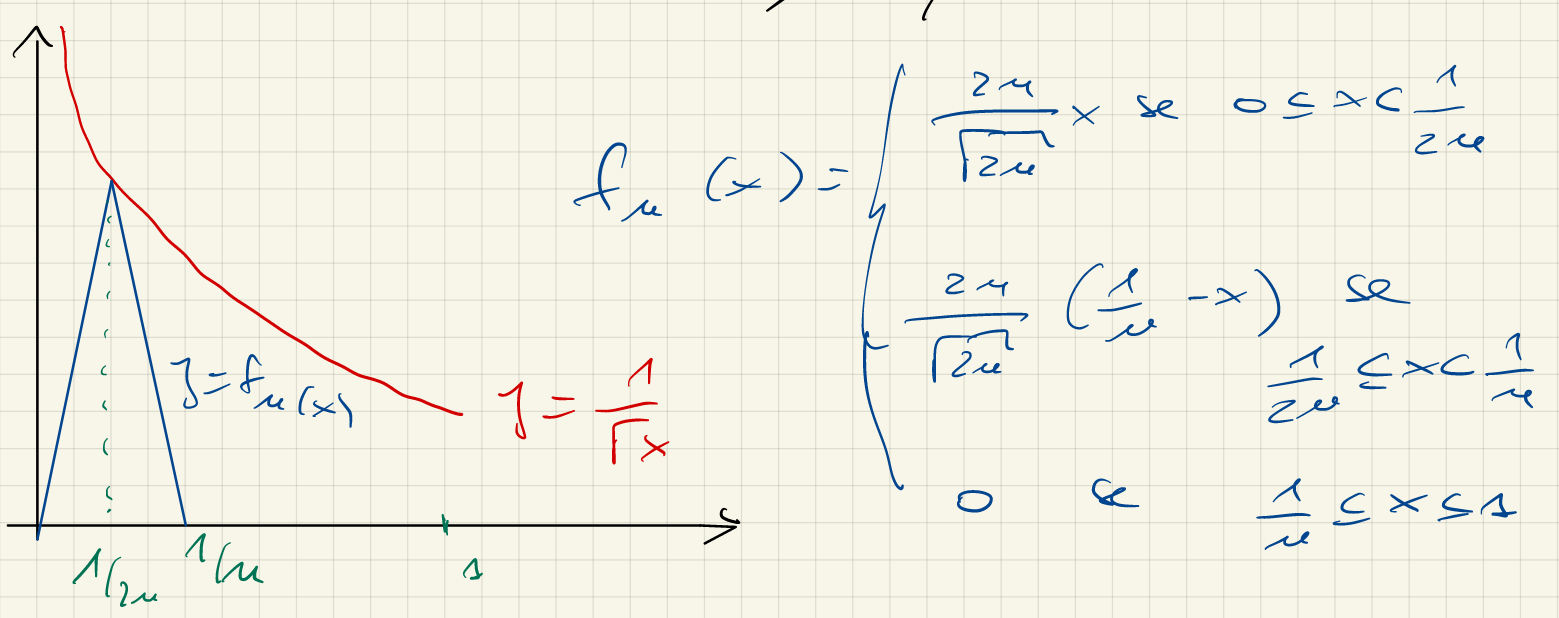
\includegraphics[width=0.7\textwidth]{Screenshot from 2023-03-28 20-48-27}
	\end{figure}
	
	$\parallel f_n \parallel_\infty = \sqrt{2n}\rightarrow +\infty$ se $n\rightarrow +\infty$, $f_n \in K$
	\item $C^\circ ([0,1]), \{f_n\}_{n\geq 1}$ come sopra. Allora $f_n \rightarrow f=0$ per $\parallel \cdot \parallel_1$\\
	$\parallel f_n -0 \parallel_1 =\int_{0}^{1} |f(x)|dx =\frac{1}{n} \sqrt{2n}\frac{1}{2}= \frac{1}{\sqrt{2n}} \rightarrow 0$ per $n \rightarrow +\infty$\\
	Ma $\parallel f_n -0 \parallel_\infty = \sqrt{2n} \rightarrow +\infty \Rightarrow f_n \nrightarrow 0$ per $\parallel \cdot \parallel_\infty$
\end{itemize}


\paragraph{\textcolor{red}{Osservazione}}
$K \subseteq \R^n$ è limitato per $|\cdot| \Leftrightarrow$ lo è per $\parallel \cdot \parallel_\infty \Leftrightarrow$ lo è per $\parallel \cdot \parallel_1$\\
$\parallel \overline{x} \parallel_\infty \leq |\overline{x}|\leq \parallel \overline{x} \parallel_1 \leq n \parallel\overline{x} \parallel_\infty$\\
\begin{figure}[!h]
	\centering
	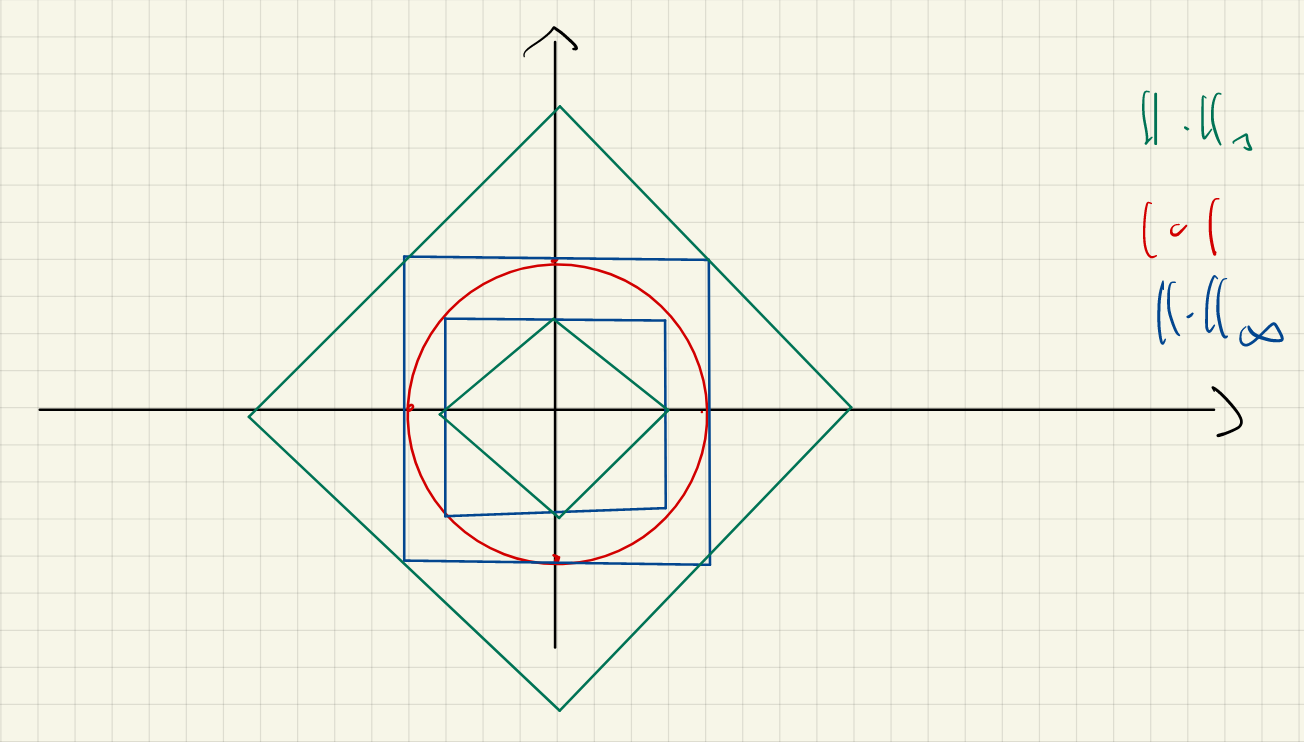
\includegraphics[width=0.7\textwidth]{Screenshot from 2023-03-28 20-55-22}
\end{figure}

\paragraph{\textcolor{red}{Osservazione}}
Introduciamo in $\R^n$ il simbolo $\infty$. Un intorno di $\infty$ è un qualunque insieme $A \subseteq \R^n$ tale che $A$ contiene il complementare di una palla di centro l'origine, cioè $\exists R>0$ tale che $\overline{x} \in A \Rightarrow \parallel \overline{x} \parallel > R$\\
\begin{figure}[!h]
	\centering
	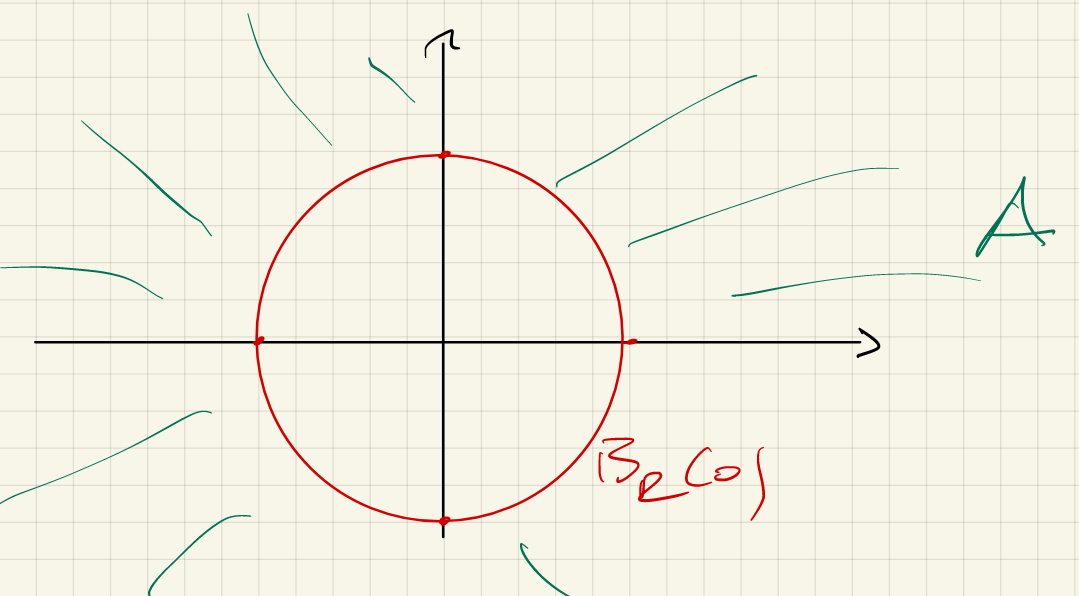
\includegraphics[width=0.5\textwidth]{Screenshot from 2023-03-28 21-04-48}
\end{figure}

Una successione $\{\overline{x_k}\}_{k\geq 1} \subseteq \R^n$ si dice divergente a $\infty$ e si scrive $\lim_{k \rightarrow \infty} \overline{x_k}=\infty$ se $\lim_{k \rightarrow \infty} |\overline{x_k}|=+\infty$ cioè se $\forall\,\, R > 0\,\, \exists\, N >0\,\,|\,\,k>N \Rightarrow |\overline{x_k}|>R$

\paragraph{\textcolor{red}{Esempio}}
$\overline{x_k}=(e^{-k},2+\frac{1}{k},\ln k) \subseteq \R^3,\,\, k \geq 1$\\
$\lim_{k}x_{k1}=\lim_{k}e^{-k}=0$\\
$\lim_{k}x_{k2}=\lim_{k}2+\frac{1}{k}=2$\\
$\lim_{k}x_{k3}=\lim_{k}\ln k=+\infty$\\
$\lim_{k}|\overline{x_k}|=\lim_{k} \sqrt{e^{-2k}+(2+\frac{1}{k})^2+(\ln k)^2} = +\infty \Rightarrow \lim_{k} \overline{x_k}=\infty$

\subsection{\textcolor{red}{Limiti di Funzione}}
\paragraph{\textcolor{red}{Definizione}}
$(X,d)$ spazio metrico, $A \subseteq X$, non vuoto. $x_0 \in X$ si dice \textcolor{red}{punto di accumulazione} per $A$ se  $\forall \epsilon >0 \,\, \exists \,\, x \in A, x \neq x_0,$ tale che $x \in B_\epsilon(x_0)$, cioè se $B_\epsilon (x_0) \cap A$ contiene punti di $A$ diversi da $x_0$. $x_0 \in A$ si dice \textcolor{red}{punto isolato} se non è di accumulazione, cioè se $\exists \epsilon >0$ tale che $B_\epsilon (x_0) \cap A =\{x_0\}$.

\paragraph{\textcolor{red}{Definizione}}
$(X,d_x),(Y,d_y)$ spazi metrici, $f:dom f \rightarrow Y$, con $domf \subseteq X, x_0 \in X $ punto di accumulazione per $domf$. Si dice che $f$ ha limite $l \in Y$ per $x \rightarrow x_0$ e si scrive
\begin{empheq}{equation*}
	\lim_{x \rightarrow x_0} f(x)=l \,\,\,\,\,\, \text{oppure} \,\,\,\,\,\, f(x) \rightarrow l \,\,\,\, \text{per} \,\,\, x \rightarrow dx_0
\end{empheq}
se per ogni intorno  $V$ di $l$  esiste un intorno $U$ di $x_0 $ tale che $ f(x) \in V$, $x \in U \cap domf, x \neq x_0$\\
In altre parole, $\lim_{x \rightarrow x_0} f(x) =l\,\,\forall\,\, \epsilon >0 \,\ \exists \,\, \delta >0 \,\,|$ se $0 < d(x,x_0) < \delta$ e $x \in domf $, allora $d_y(f(x),l)<\epsilon$\\
\textcolor{orange}{Se prendo la definizione data con $\epsilon$ e $\delta$ per $X=Y=\R$ e le distanze $d_x(x,y)=d_y(x,y)=|x-y|$, ottengo la definizione con $\epsilon$ e $\delta$ data in ambito reale.}

\paragraph{\textcolor{red}{Teorema di unicità del limite}}
$(X,d_x)$ e $(Y,d_y)$ spazi metrici, $f: domf \rightarrow Y$, $domf \subseteq X, x_0 \in X$ punto di accumulazione per $domf$.\\
Se $\lim_{x \rightarrow x_0} f(x) = l_1 \in Y$ e $\lim_{x \rightarrow x_0} f(x) = l_2 \in Y$, allora $l_1=l_2$.

\paragraph{\textcolor{red}{Proposizione}}
$(X,d)$ spazio metrico, $\overline{f}: dom\overline{f} \rightarrow \R^n,\,\, \overline{f}(x)=(f_1(x),...,f_n(x))$, $x_0 \in X$ punto di accumulazione per $dom \overline{f} \subseteq X$, allora $\lim_{x \rightarrow x_0} \overline{f}(x)=\overline{l}=(l_1,...,l_n)\in \R^n \Leftrightarrow \lim_{x \rightarrow x_0} f_j(x)=l_j \forall j=1,2,...,n$.

\paragraph{\textcolor{red}{Teorema della permanenza del segno}}
$(X,d)$ spazio metrico, $f: domf \rightarrow\R$, $domf \subseteq X, x_0 \in X$ punto di accumulazione per $domf$.\\
Se $\lim_{x \rightarrow x_0} f(x) = l >0$, allora $f(x)>0$ definitivamente per $ x \rightarrow x_0$, cioè $\exists \,\, \delta >0 \,\, |\,\, f(x)>0 \,\, \forall \,\, x \in B_\delta (x_0)\cap domf$, $x \neq x_0$. 

\paragraph{\textcolor{red}{Teorema}}
$(X,d)$ spazio metrico, $f,g: A \rightarrow\R$, $A \subseteq X, x_0 \in X$ punto di accumulazione per $A$, tali che $\lim_{} f(x) =l_f$, $\lim_{x \rightarrow x_0} g(x)=l_f$ e $f(x)\leq g(x)$ definitivamente per $x \rightarrow x_0$. \\\textcolor{orange}{$\exists \delta > 0 | f(x) \leq g(x) \forall x \in B_\delta (x_0) \cap A$, $x \neq x_0$.)}\\ Allora $l_f \leq l_g$.

\paragraph{\textcolor{red}{Teorema del Confronto}}
$(X,d)$ spazio metrico, $f,g,h : A \rightarrow \R, A \subseteq X, x_0$ punto di accumulazione per $A$, tali che $g(x) \leq f(x)\leq h(x)$ definitivamente per $x \rightarrow x_0$. Se $\lim_{x \rightarrow x_0} g(x)=\lim_{x \rightarrow x_0} h(x)=l$, allora $\lim_{x \rightarrow x_0} f(x)=l$.

	
	
	
\end{comment}